i% LaTeX template for Science journal paper
% Based on science_template.tex with adaptations for research content

%%%%%%%%%%%%%%%% START OF PREAMBLE %%%%%%%%%%%%%%%

% Basic setup. Authors shouldn't need to adjust these commands.
% They need to be included in this .tex for Science's production software to work.

% Use the basic LaTeX article class, 12pt text
\documentclass[12pt]{article}

% Science uses Times font. If you don't have this installed, comment out the following line
\usepackage{newtxtext,newtxmath}
% Depending on your LaTeX fonts installation, you might get better results with one of these:
%\usepackage{mathptmx}
%\usepackage{txfonts}

% Allow external graphics files
\usepackage{graphicx}


\usepackage{booktabs}
\usepackage{tabularx}
% Use US letter sized paper with 1 inch margins
\usepackage[letterpaper,margin=1in]{geometry}

% Double line spacing, including in captions
\linespread{1.5} % For some reason double spacing is 1.5, not 2.0!

% One space after each sentence
\frenchspacing
\usepackage[dvipsnames]{xcolor}
\definecolor{lightblue}{rgb}{0.68,0.85,0.9}

% Abstract formatting and spacing - no heading
\renewenvironment{abstract}
	{\quotation}
	{\endquotation}

% No date in the title section
\date{}

% Reference section heading
\renewcommand\refname{References and Notes}

% Figure and Table labels in bold
\makeatletter
\renewcommand{\fnum@figure}{\textbf{Figure \thefigure}}
\renewcommand{\fnum@table}{\textbf{Table \thetable}}
\makeatother
\renewcommand\refname{References and Notes}
\makeatletter
\renewcommand{\fnum@figure}{\textbf{Figure \thefigure}}
\renewcommand{\fnum@table}{\textbf{Table \thetable}}
\makeatother
\usepackage{scicite}
\usepackage{url}
\usepackage{tikz}
%\newcommand{\aladyn}{\texttt{ALADYNOULLI}}
\newcommand{\aladyn}{\texttt{ALADYNOULLI}}
\usepackage{tikz}
\usepackage{amsmath}
\let\Bbbk\relax
\usepackage{amssymb}
\usepackage{geometry}
\geometry{margin=1in}
% Call the accompanying scicite.sty package.
% This formats citation numbers in Science style.
\usepackage{scicite}

% Provides the \url command, and fixes a crash if URLs or DOIs contain underscores
\usepackage{url}

\usepackage{setspace}
\usepackage{caption}
\captionsetup{font={singlespacing}}

%%%%%%%%%%%% CUSTOM COMMANDS AND PACKAGES %%%%%%%%%%%%

% Authors can define simple custom commands e.g. as shortcuts to save on typing
% Use \newcommand (not \def) to avoid overwriting existing commands.


%%%%%%%%%%%%%%%% TITLE AND AUTHORS %%%%%%%%%%%%%%%%

% Title of the paper.
% Keep it short and understandable by any reader of Science.
% Avoid acronyms or jargon. Use sentence case.
\def\scititle{
	\aladyn: A Bayesian approach to disease progression modeling for genomic discovery and clinical prediction
}
% Store the title in a variable for reuse in the supplement (otherwise \maketitle deletes it)
\title{\bfseries \boldmath \scititle}

% Author and institution list.
% Institution numbers etc. should be hard-coded, do *not* use the \footnote command.
\author{
    Sarah M. Urbut$^{1,2,3,4}$,
    Yi Ding$^{5}$,
    Tetsushi Nakao$^{1,2,4}$,
    Xilin Jiang$^{6}$,\and
    Leslie Gaffney$^{4}$,
    Anika Misra$^{1,2,4}$,
    Whitney Hornsby$^{1,2,4}$,
    Jordan W. Smoller$^{3,4,7,8}$\and
    Alexander Gusev$^{5,3,4\dagger}$,
    Pradeep Natarajan$^{1,2,3,4\dagger}$,
    Giovanni Parmigiani$^{9,10\dagger}$\and
    % Institution list, in a slightly smaller font
    \small$^{1}$Division of Cardiology, Department of Medicine, Massachusetts General Hospital, Boston, MA 02114, USA\and
    \small$^{2}$Cardiovascular Research Center, Massachusetts General Hospital, Boston, MA 02114, USA\and
    \small$^{3}$Harvard Medical School, Boston, MA 02215, USA\and
    \small$^{4}$Broad Institute of Harvard and MIT, Cambridge, MA 02142, USA\and
    \small$^{5}$Division of Population Sciences, Dana-Farber Cancer Institute, Boston, MA 02215, USA\and
    \small$^{6}$University of Cambridge, Cambridge, UK\and
    \small$^{7}$Psychiatric and Neurodevelopmental Genetics Unit, Center for Genomic Medicine, \\ \small Massachusetts General Hospital, Boston, MA 02114,USA\and
    \small$^{8}$Department of Epidemiology, Harvard TH Chan School of Public Health, Boston, MA 02115, USA\and
    \small$^{9}$Department of Biostatistics, Harvard TH Chan School of Public Health, Boston, MA 02115, USA\and
    \small$^{10}$Department of Data Science, Dana-Farber Cancer Institute, Boston, MA 02215, USA\and    
    % Identify at least one corresponding author, with contact email address
    \small$^\ast$Corresponding author. Email: gp@jimmy.harvard.edu\and
    % Joint contributions can be indicated like this
    \small$^\dagger$These authors jointly supervised this work.
}
%%%%%%%%%%%%%%%%% END OF PREAMBLE %%%%%%%%%%%%%%%%


%%%%%%%%%%%%%%%% START OF MAIN TEXT %%%%%%%%%%%%%%%
\begin{document} 

% Insert the title and author list
\maketitle

% Abstract, in bold

\begin{abstract} \bfseries \boldmath
Understanding how disease patterns evolve over a lifetime remains a key challenge in medicine. While electronic health records provide rich longitudinal data, existing models typically analyze each disease in isolation, missing the complex interplay between multiple conditions and genetic factors. Here, we combine longitudinal health records with genetic data to model individual trajectories, using a novel latent dynamic Bayesian framework called $\aladyn$ that identifies latent disease signatures from longitudinal health records while modeling individual-specific trajectories. Applied across three biobanks with up to 50 years of follow-up, our model discovers clinically interpretable disease signatures that demonstrate remarkable consistency across diverse populations (79.2\% cross-cohort correspondence) and show strong genetic correlations, enabling both accurate prediction of patient risk and discovery of novel genetic associations. The model achieves dramatic improvements in disease prediction across 24 conditions (median dynamic AUC 0.85, gains up to 0.20), outperforming established clinical risk scores across diverse conditions. Furthermore, our signature-based approach identifies 150 novel genetic loci missed by single-disease GWAS, with multiple signatures showing strong genetic signals (cardiovascular h² = 0.041, musculoskeletal $h^{2}$ = 0.035). Critically, this unified modeling approach significantly improves predictive performance for multiple diseases while revealing distinct biological subtypes within traditional diagnostic categories—demonstrating substantial heterogeneity across diverse conditions including cancer, metabolic disorders, and psychiatric conditions, with Cohen's d effect sizes up to 3.87 for signature differences between patient clusters ($p \leq 1\times 10^{8}$ for 95\% of comparisons). In conclusion, $\aladyn$ combines genetics and longitudinal diagnosis to achieve both improved disease prediction and enhanced genetic discovery through a unified framework that captures the complex interplay between genetic predisposition and time-varying disease patterns.
\end{abstract}

\section*{Introduction}

% The first paragraph does NOT have a heading
\noindent


The risk of disease varies substantially between individuals and throughout life, with complex interactions between genetic predisposition, environmental factors, and accumulated comorbidities. Understanding these dynamic patterns of risk could transform early detection, prevention, and personalized treatment strategies \cite{berry_bayesian_2006,bellot_flexible_2020,angus_heterogeneity_2021}. The increasing availability of large-scale electronic health records (EHRs) linked to genetic data provides unprecedented opportunities to model these complex disease trajectories at a population scale \cite{sudlow_uk_2015, pedersen_adult_2023}. However, extracting meaningful patterns from these rich, longitudinal datasets remains challenging due to patient population heterogeneity, the temporal nature of disease progression, and intricate relationships between diverse conditions.

Traditional approaches to analyzing EHR data often focus on isolated diseases or simple pairwise associations, failing to capture how multiple conditions evolve together over time \cite{wang_empirical_2021}. Recent unsupervised methods have attempted to identify disease clusters or trajectories \cite{jiang_age-dependent_2023}, but typically do not account for temporal dynamics of disease risk or individual-level heterogeneity, particularly the influence of genetic factors on disease progression rates \cite{urbut_dynamic_2023, hyttinen_genetic_2003}. Furthermore, many models assume conditional independence of diseases, missing the opportunity to leverage information across related conditions for both prediction and discovery \cite{blei_dynamic_2006, blei_latent_2003}. Consider a patient who develops rheumatoid arthritis at age 45, followed by hypertension at 48, and eventually suffers a myocardial infarction at 52. Traditional approaches may treat these as separate events or simple comorbidities, missing the underlying metabolic-inflammatory signature that drives this progression. Also, they do not typically leverage information from patients with similar patterns to improve prediction for rare conditions, where limited data makes traditional disease-specific models less reliable.

We present $\aladyn$, a generative model that integrates genetic data with longitudinal EHRs to identify latent disease signatures while modeling individual-specific health trajectories over time.  $\aladyn$ addresses these limitations by identifying shared disease signatures that capture biological pathways common across multiple conditions, enabling more accurate prediction even for rare diseases through information sharing with related, more common conditions. Our approach offers several key advantages over existing methods: (1) \textbf{Interpretability}: disease signatures correspond to clinically meaningful biological processes rather than abstract statistical factors; (2) \textbf{Temporal modeling}: captures how disease risk evolves dynamically over the life course rather than static risk assessment; (3) \textbf{Genetic integration}: directly incorporates genetic information into the model architecture rather than as post-hoc analysis; (4) \textbf{Unified framework}: simultaneously models multiple diseases, sharing information across related conditions and improving prediction even for diseases with sparse data \cite{caruana_multitask_1997}; and (5) \textbf{Individual-specific trajectories}: provides personalized risk profiles that adapt as new clinical information becomes available. By jointly modeling multiple diseases and their genetic determinants, $\aladyn$ enables both improved prediction of future disease risk and enhanced discovery of genetic architecture underlying complex phenotypes, while revealing meaningful patient subgroups with distinct biological mechanisms that could inform personalized interventions.

% Research Articles split the text into sections using descriptive headings
\section*{Results}
\subsection*{$\aladyn$ captures temporal disease signatures and individual trajectories}

Disease patterns among individuals vary by onset, progression speed, and composition, reflecting different underlying biological mechanisms. Unlike allocation-based topic models that conditionally allocate observed diseases to categories \cite{jiang_age-dependent_2023, blei_dynamic_2006}, $\aladyn$  models the probability of each disease for an individual by integrating across multiple latent signatures (\textbf{Figure~\ref{fig:model_overview})}.

For each individual $i$, disease $d$, and time point $t$, we model the probability of disease occurrence $\pi_{idt}$ as a weighted combination of signature-specific probabilities, where each signature captures patterns of diseases that tend to occur together (\textbf{Table~\ref{tab:notation})}:

\begin{equation}
\pi_{idt} = \kappa \cdot \sum_{k=1}^{K} \theta_{ikt} \cdot \text{sigmoid}(\phi_{kdt}),
\label{eq:pieqn}
\end{equation}

\noindent where $\text{sigmoid}(\phi_{kdt}) = 1/(1+e^{-\phi_{kdt}})$, $\kappa$ is a global calibration parameter, $\theta_{ikt}$ represents a normalized individual $i$'s time-varying association with signature $k$ at time $t$, and $\phi_{kdt}$ captures the relationship between signature $k$ and disease $d$ over time $t$.

The normalized individual-signature associations (loadings) $\theta_{ikt}$ are derived from latent variables $\lambda_{ikt}$ through a softmax transformation:

\begin{equation}
\theta_{ikt} = \frac{\exp(\lambda_{ikt})}{\sum_{k'=1}^{K} \exp(\lambda_{ik't})}.
\label{eq:theta_gp}
\end{equation}

These latent variables $\lambda_{ikt}$ follow a Gaussian process \cite{Rasmussen2006Gaussian} prior wherein we model the effects of genetic factors and time (see \textbf{Methods; Figure~\ref{fig:training_architecture})}. Specifically:

\begin{equation}
\lambda_{ik} \sim \mathcal{GP}(r_k + \mathbf{g}_i^{\top}\Gamma_k, \Omega_{\lambda})
\label{eq:lambda_gp}
\end{equation}


\noindent where $r_k$ is a signature-specific reference level, $\Gamma_k$ captures genetic effects on signature predisposition, $\mathbf{g}_i$ represents individual genetic factors, here polygenic scores, affecting the mean of $\lambda_{ik}$, and $\Omega_{\lambda}$ is a temporal covariance kernel modeling smooth trajectories for $\lambda_{ikt}$ over time.

Similarly, the disease-signature associations follow a Gaussian process prior:

\begin{equation}
\phi_{kd} \sim \mathcal{GP}(\mu_d + \psi_{kd}, \Omega_{\phi})
\label{eq:phi_gp}
\end{equation}

\noindent where $\mu_d$ is a disease-specific baseline, or the logit of the population prevalence, $\psi_{kd}$ represents the overall strength of association between signature $k$ and disease $d$, and $\Omega_{\phi}$ allows for temporal variation in these associations.

A key innovation of our approach lies in its formulation as a mixture of probabilities rather than a probability of a mixture, as in traditional sparse factor analysis approaches \cite{wang_empirical_2021}. Unlike allocation-based topic models that conditionally assign diseases to individuals $\textit{after}$ the event has necessarily occurred \cite{jiang_age-dependent_2023}, $\aladyn$ directly models the probability of disease occurrence as a weighted combination of signature-specific disease probabilities.

This crucial distinction allows our model to: (1) predict future disease onset rather than merely explain observed diagnoses; (2) accommodate multiple contributing disease processes simultaneously rather than forcing competitive allocation to a single signature; and (3) accurately model chronic conditions that persist over time rather than treating each diagnosis as an independent event. The combination of softmax-transformed individual loadings ($\theta$) and sigmoid-transformed disease probabilities ($\phi$) ensures proper probability scaling.

\textbf{Terminology clarification:} We note that factor analysis literature exhibits inconsistent terminology that can be confusing. In some traditions (e.g., sparse factor analysis \cite{wang_empirical_2021, engelhardt_analysis_2010}), "loadings" refer to individual-specific weights (our $\lambda$ parameters), while "factors" or "coefficients" refer to feature importance (our $\phi$ parameters). In other traditions, "loadings" refer to feature importance (our $\phi$ parameters), while individual components are called "scores" or "weights" (our $\lambda$ parameters). Throughout this work, we use "loadings" to refer to individual-specific signature associations ($\lambda$ and $\theta$) and "signature-disease associations" to refer to feature importance ($\phi$), consistent with the sparse factor analysis convention where loadings represent individual variation and factors represent feature structure.

\textbf{Two complementary applications:} $\aladyn$ serves two distinct but complementary purposes, each requiring different analytical approaches. For biomedical discovery, $\aladyn$ operates with complete hindsight, leveraging entire patient trajectories to maximize our ability to identify biological patterns and mechanisms. This retrospective analysis transforms our understanding of disease patterns, progression speed, genetic relationships, and disease associations by using all available longitudinal data to characterize disease signatures, quantify genetic influences, and reveal patient heterogeneity within diagnostic categories. For clinical prediction, we operate under strict temporal constraints that mirror real-world clinical decision making (see \textbf{Figure~\ref{fig:training_architecture}} for distinction). We employ a rigorous temporal validation framework that uses only information available up to a prediction time point (see \textbf{Figure ~\ref{fig:recruitment_timeline}}). This prospective approach simulates real-world clinical scenarios where physicians must predict future risk based solely on a patient's history to date, ensuring our performance metrics reflect true predictive capability rather than retrospective explanation.



\subsection*{Applying $\aladyn$ identifies consistent signature patterns across diverse populations}

We applied $\aladyn$ to three independent cohorts: UK Biobank (UKB, n=427,239), Mass General Brigham (MGB, n=48,069), and All of Us (AoU, n=208,263) (\textbf{Table~ \ref{tab:baseline_characteristics}, Figure~\ref{fig:cohort_design}}). We obtained ICD-10 codes from hospitalization diagnoses in each biobank \cite{sudlow_uk_2015, koyama_decoding_2023} and transformed these to pheCodes \cite{bastarache_using_2021}, following established approaches for EHR phenotyping \cite{hripcsak_next-generation_2013} (see \textbf{Methods}). A set of 348 pheCodes were selected representing diseases with at least 1000 unique occurrences in UK Biobank hospitalization episode statistics \cite{yeung_ukbpheno_2022} as in \cite{jiang_age-dependent_2023}. Despite differences in population characteristics, healthcare systems, and data collection methodologies across these cohorts, our model identified remarkably consistent signature patterns (\textbf{Table\ref{tab:signature_summary_actual}; Figure~\ref{fig:cluster_correspondence})}.


We set K=20 for our model, which converged well (\textbf{\ref{fig:phi_batch}}) across all three biobanks and successfully identified 20 distinct disease signatures from the data. These model-derived signatures corresponded to recognized disease processes and captured diverse disease domains including cardiovascular, metabolic, pulmonary, psychiatric, musculoskeletal, and oncologic conditions (\textbf{\ref{tab:signature_summary_actual}}). Each signature demonstrates characteristic temporal patterns, with disease probabilities evolving dynamically with age across biobanks (\textbf{Figure~\ref{fig:signature-dynamics}A; Figures~\ref{fig:temporal_ukb},~\ref{fig:temporal_aou},~\ref{fig:temporal_mgb})}. For example, the cardiovascular signature shows steadily increasing probabilities for conditions like atrial fibrillation and heart failure after age 55 years, while the malignancy signature displays a sharp rise in metastatic disease probabilities between ages 60-75 years. The specificity of each signature for a given disease, as modeled by $\psi_{kd}$, is preserved but heterogeneous, reflecting the model's ability to disentangle signature-disease specificity (\textbf{Figure~\ref{fig:signature-dynamics}B)}.

Furthermore, the model's tensor structure (\textbf{Figure~\ref{fig:data-description})}, enables rapid disease hazard calculation using the average loadings (\textbf{Equation~\ref{eq:lambda_gp}}) and population-level $\phi_{kd}$. The average age-specific hazard probabilities for a wide range of diseases are visualized in \textbf{Figure~\ref{fig:signature-dynamics}C}, highlighting temporal risk patterns.


As stated, these signature patterns show strong consistency across the three independent cohorts (\textbf{Figure~\ref{fig:signature-dynamics}D,  Figures~\ref{fig:temporal_ukb},~\ref{fig:temporal_aou},~\ref{fig:temporal_mgb})}. When comparing the membership of diseases within signatures between any two cohorts, we observed high concordance (median modified Jaccard index = 0.792, IQR = 0.65-0.89 across all pairwise comparisons between biobanks for similarity-matched signatures when computing intersection among signatures normalized to total number of diseases within the matched UKB signature, \textbf{Figure ~\ref{fig:cluster_correspondence})}. \textbf{Figure~\ref{fig:signature-dynamics}E} illustrates this consistency for two key signatures: cardiovascular disease and malignancy. Despite differences in healthcare systems and coding practices, the temporal patterns of key diseases within these signatures remain remarkably consistent, supporting the biological validity of the discovered patterns.

The model also captures disease-specific temporal dynamics that match clinical expectations. For instance, Type 1 diabetes peaks earlier in life compared to Type 2 diabetes within the metabolic signature (\textbf{Fig \ref{fig:signature-dynamics}E}), while primary malignancies precede metastatic disease within the cancer signature. These nuanced temporal relationships emerge directly from the model without explicit encoding, demonstrating $\aladyn$'s ability to learn clinically meaningful disease trajectories.



\subsection*{Personalized trajectories reveal heterogeneity within disease categories}
Beyond population-level signatures, $\aladyn$ provides individual-specific trajectory information through the time-varying $\lambda_{ikt}$ parameters that reveal distinct disease progression patterns. 

While each patient in \textbf{Figures \ref{fig:individual_trajectories}A-C} demonstrate similar average signature loadings in aggregate (horizonal 'static model summary' profile), their disease journeys reveal biological differences among patients sharing this diagnosis, reflecting true heterogeneity—i.e., the presence of distinct subgroups with different underlying disease signature distributions—within the diagnostic category. Patient C (Panel C) experiences MI at age 54 following a complex trajectory of gastrointestinal and musculoskeletal conditions, with cardiovascular signature activation beginning subtly around age 50 and accelerating dramatically in the years preceding the event. In contrast, Patient B (Panel B) develops MI at age 72 after a markedly different prodrome dominated by respiratory and dermatologic conditions, showing a more gradual cardiovascular signature evolution. Post-MI trajectories in these two patients also diverge substantially: Patient C subsequently develops multiple cardiovascular complications and metabolic disorders, while Patient B's post-MI course is characterized by different comorbidity patterns including genitourinary and infectious disease manifestations. These distinct temporal signatures preceding and following identical clinical endpoints illustrate how $\aladyn$ captures the biological heterogeneity masked by traditional diagnostic categories—revealing that "myocardial infarction" encompasses diverse pathophysiological pathways that may require different prevention and treatment strategies. Multiple additional examples (\textbf{Figure ~\ref{fig:patient_trajectories})} demonstrate the diversity in temporal loadings that would be missed by a summative approach considering only average loading.

Our model also illustrates how individual-level trajectories and population phenomena combine to elicit time-varying personalized disease probabilities. {\textbf{Figure~\ref{fig:individual_trajectories}E}} is a heatmap of log disease probabilities by signature and age for MI, showing how overall MI risk is decomposed into the contributions of various time-varying signature loadings. This visualization reveals the complex interplay between multiple signatures in determining disease risk. While the cardiovascular signature contributes most significantly to MI risk, other signatures—particularly those related to metabolic conditions and inflammation—also play important roles. The stacked area plot below demonstrates how these contributions integrate to form the aggregate risk profile, revealing periods of accelerated risk accumulation that may represent critical windows for preventive intervention.

Aggregating these individual patterns reveals distinct group-level differences. In a retrospective analysis, the comparison of early-onset ($\leq$ 55 years, mean age of event 49.7 years) and late-onset ($\geq$ 70 years, mean age of onset 74.9 years) MI in \textbf{Figure~\ref{fig:individual_trajectories}D} shows that early-onset patients exhibit a higher and earlier peak in cardiovascular signature contribution, as well as a more rapid increase in signature loading prior to the event, compared to late-onset cases. These quantitative differences in trajectory characteristics suggest that early- and late-onset MI, while sharing the same clinical diagnosis, may represent distinct disease entities requiring different preventive strategies.


This pattern of heterogeneity within diagnostic categories extends broadly across diseases. \textbf{Figure~\ref{fig:individual_trajectories}F} captures signature heterogeneity within disease subtypes through stacked area plots showing deviations from the population average, highlighting the diversity of underlying biological processes among patients sharing the same clinical diagnosis. 

To assess whether these signature-based heterogeneity patterns represent fundamental biological variation rather than cohort-specific artifacts, we examined the consistency of signature deviation patterns across biobanks. For patients with a given disease (e.g., myocardial infarction, breast cancer, major depressive disorder), we computed signature-specific deviations from population-average loadings and found remarkable concordance in these deviation patterns across UK Biobank, Mass General Brigham, and All of Us cohorts. This cross-cohort consistency in patient heterogeneity demonstrates that signature-based patient characterization captures fundamental biological variation that transcends population differences, healthcare systems, and coding practices. The ability to identify consistent patient subgroups with shared signature profiles across diverse populations validates the biological meaningfulness of our approach and suggests that signature-based stratification could be generalizable across healthcare settings.

To systematically quantify differences in signature composition among patients with the same clinical diagnosis for three representative diseases (myocardial infarction, breast cancer, and major depressive disorder), we applied k-means clustering to patients' time-averaged signature loadings for each disease (\textbf{Figure~\ref{fig:individual_trajectories}F)} 
%This approach identifies distinct subgroups of patients who share similar underlying disease signature profiles despite having the same clinical diagnosis. 
\newcommand{\Ccsig}{$C_{ck}^{\mbox{\small SIG}}$ }
We then calculated cluster-specific Cohen's effect sizes\cite{cohen_statistical_2013} \Ccsig as follows (\textbf{Figure \ref{fig:cohen_d}; Extended data Data S1-S3)}. For cluster $c$ and  signature $k$, \Ccsig is the standardized difference in mean time-averaged signature loadings between individuals in cluster $c$ and those in all other clusters (see \textbf{Figure~\ref{fig:cohen_d})}. This measures of how distinct each cluster is with regard to each disease signature. %This analysis revealed substantial standardized differences in signature loadings between patient subgroups, reflecting biological processes not typically considered in diagnoses.

%To then further quantify the biological heterogeneity within each disease, we calculated Cohen's $d$ effect sizes and corresponding p-values for the difference in time-averaged signature loadings between clusters, across all signatures and for each of the three representative diseases (myocardial infarction, breast cancer, and major depressive disorder). 
This analysis revealed that the vast majority of signature differences between clusters were not only large in magnitude (with many \Ccsig values exceeding 0.8, and some as high as 2.5–3.9), but also highly statistically significant (p $\leq 1\times$10$^{-8}$ for nearly all clusters). The largest effect size occurs in major depressive disorder, for the acute illness signature 16 (septicemia, acute renal failure, and critical care conditions) in cluster 2 showed $C_{2,16}^{\mbox{\small SIG}} = 3.87$ (p $\approx$ 0), revealing a medically complex depression subgroup with severe acute comorbidities. In myocardial infarction, the cardiovascular signature 5 (encompassing coronary atherosclerosis, ischemic heart disease, and hypercholesterolemia) shows $C_{3,5}^{\mbox{\small SIG}} = 2.86$ (p $\approx$ 0) in only one cluster, indicating that even within cardiovascular diseases, the cardiovascular signature itself reveals substantial heterogeneity between patient subgroups. In breast cancer, the cardiovascular signature also showed strong differentiation ($C_{3,5}^{\mbox{\small SIG}}$ = 2.46, p $\approx$ 0). Similarly, the pain/inflammatory/metabolic signature (Signature 7, characterized by asthma, migraine, osteoporosis, depression, and obesity) achieved near-complete patient separation in all conditions examined, with $C^{\mbox{\small SIG}}$ values ranging from 1.84 to 2.51. These effect sizes indicate near-complete separation between patient subgroups, suggesting distinct underlying disease processes within the same diagnostic category, underscoring the presence of distinct biological subgroups within each diagnostic category. These results demonstrate that the observed heterogeneity is both quantitatively substantial and statistically robust, supporting the biological relevance of the patient subgroups we identified (see \textbf{Extended Data S1-S3}). 

To further demonstrate biological heterogeneity within disease categories, we performed a comprehensive pathway analysis for myocardial infarction using deviation-from-reference clustering, which identifies distinct biological pathways leading to the same clinical outcome (\textbf{Extended Data Figure S28}). This analysis revealed four distinct pathways to MI, each representing different proportions of patients (7.4\%, 44.8\%, 17.9\%, and 29.9\%) with distinct signature activation patterns, disease associations, and genetic risk profiles. Pathway-specific analyses showed that different pathways exhibit distinct precursor disease patterns (e.g., Pathway 0 shows 86.3\% prevalence of coronary atherosclerosis before MI, compared to population reference of 5.4\%), signature deviation trajectories, and enrichment of familial hypercholesterolemia carriers (Pathway 0: 1.92× enrichment). Cross-cohort validation demonstrated remarkable reproducibility of these pathways between UK Biobank and Mass General Brigham cohorts, confirming that signature-based pathway identification captures fundamental biological variation that transcends healthcare systems and coding practices. This pathway-level heterogeneity analysis complements the patient-level clustering described above, demonstrating that "myocardial infarction" encompasses multiple distinct biological entities with different underlying mechanisms, genetic determinants, and clinical trajectories.

The model's ability to identify such distinct temporal trajectories and biological subtypes even among patients with similar diagnoses illustrates $\aladyn$'s potential for personalized risk assessment and intervention timing (\textbf{Figure~\ref{fig:patient_trajectories})}. By capturing how an individual's signature associations evolve with each new diagnosis, $\aladyn$ provides a dynamic framework for monitoring disease progression, predicting future complications, and identifying optimal windows for preventive measures. Unlike traditional risk scores that provide a single probability estimate, $\aladyn$ offers a comprehensive view of an individual's evolving disease landscape—revealing not just what conditions might develop but when and in what sequence—critical information for precision medicine.


\subsection*{Genetic factors influence signature trajectories}

A key innovation of $\aladyn$ is its integration of genetic information directly into the model, allowing us to quantify how genetic factors influence disease signature associations. We examined both the direct genetic effects on signature loadings through the $\Gamma_k$ parameters and the association between polygenic risk scores (PRS) and signature trajectories. Importantly, to avoid double-dipping, we used external PRS that were developed independently of our signature analysis, ensuring that genetic information was not used both in training the model and in evaluating PRS-signature associations.

Genetic analysis revealed substantial genetic influence on signature associations through the $\Gamma_k$ parameters. Using batch-aggregated effect estimates across model replicates and a Bonferroni correction for 36 PRS per signature (p $\leq 6.6 \times 10^{-5}$), we identified 75 significant PRS-signature associations out of 756 tests (9.9\%) (\textbf{Fig~\ref{fig:genetics}A}; see Extended Data S0). The strongest genetic effects were observed for signatures with known heritable components: coronary artery disease PRS on the cardiovascular signature (Signature 5, $\gamma = 0.24$), LDL cholesterol PRS on Signature 5 ($\gamma = 0.11$), and type 2 diabetes PRS on the metabolic signature (Signature 15, $\gamma = 0.22$). Coronary, metabolic, and psychiatric signatures showed the strongest overall genetic influences (\textbf{Figure~\ref{fig:genetics}A}), consistent with the high heritability of these disease categories. Several PRS, including BMI, T2D, and HT, showed pleiotropic effects across multiple signatures \cite{solovieff_pleiotropy_2013}, highlighting shared genetic architecture across disease processes. Importantly, the heterogeneous patient groups identified in our trajectory analysis (\textbf{Figures~\ref{fig:individual_trajectories}D} and~\textbf{\ref{fig:individual_trajectories}F}) show corresponding heterogeneity in underlying polygenic risk scores (\textbf{Figure~\ref{fig:genetics}B}), demonstrating that genetic variation contributes to the diverse disease progression patterns we observe. 

\newcommand{\Ccprs}{$C_{cp}^{\mbox{\small PRS}}$}
We quantified the variability of PRS scores across patient clusters by computing Cohen's effect sizes \Ccprs for cluster $c$ and PRS $p$, analogously to what done earlier for signatures (see also Methods). This analysis revealed substantial differences in polygenic risk scores between patient subgroups that parallels the biological variation observed in signature loadings (\textbf{Figure \ref{fig:genetics}B; Extended Data S4-S6)} . For major depressive disorder, signature loadings showed dramatic cluster-specific effects, with Signature 16 (likely psychiatric) showing extreme enrichment in Cluster 2 ($C_{2,16}^{\mbox{\small SIG}} = 3.87$) and Signature 7 (likely inflammatory) showing strong depletion in Cluster 1 ($C_{1,7}^{\mbox{\small SIG}} = -1.37$) but enrichment in Cluster 3 ($C_{1,7}^{\mbox{\small SIG}} = 2.47$). This signature variability was mirrored by corresponding PRS patterns: Cluster 3 showed strong enrichment for cardiovascular risk factors ($C_{3,\mbox{\tiny BMI}}^{\mbox{\small PRS}} = 0.40$, $C_{3,\mbox{\tiny CVD}}^{\mbox{\small PRS}} = 0.43$, $C_{3,\mbox{\tiny CAD}}^{\mbox{\small PRS}} = 0.38$, $C_{3,\mbox{\tiny HT}}^{\mbox{\small PRS}} = 0.58$), while Cluster 2 showed depletion in these same traits (see Extended Data S4-S6).

To systematically identify genetic loci associated with signature trajectories, we performed genome-wide association studies (GWAS) on lifetime signature exposure for each signature, computed as the area under each individual's signature loading curve over their entire follow-up period (\textbf{\ref{fig:aex_calculation}; Methods}), after refitting our model excluding the genetic mean ($\mathbf{g}_i^{\top}\Gamma_k$ in Equation 3) from the prior on $\lambda$.  This approach investigates whether signature trajectories themselves have heritable components beyond the genetic effects we explicitly modeled. LD score regression analysis revealed significant SNP-based heritability for multiple signatures (Table~\ref{tab:ldsc_results}), with the strongest signal observed for the cardiovascular signature ($h^{2}$ = 0.041, SE = 0.003), followed by musculoskeletal $h^{2}$ = 0.035, SE = 0.002) and pain/inflammation signatures ($h^{2}$ = 0.027, SE = 0.002). All analyses showed appropriate genomic control ($\lambda_{gc}$ = 1.02-1.22) and negligible population stratification (intercept $\approx$ 1.0), confirming that our signatures represent biologically meaningful patterns with distinct genetic architectures.

This genetic validation analysis identified 151 genome-wide significant loci across 16 of 21 signatures, with the cardiovascular signature alone accounting for 56 loci (37\% of all discoveries) (\textbf{Extended data S7-S27} for lead variants across signatures). This signature-based approach substantially outperformed traditional single-disease GWAS in detecting disease-associated variants: our cardiovascular signature analysis identified 10 unique loci not found in any constituent trait GWAS (myocardial infarction, angina, hypercholesterolemia, coronary atherosclerosis, acute ischemic heart disease, chronic ischemic heart disease) within 1MB windows, including IL6R (rs6687726), LIPC (rs1532085), HYOU1 (rs2509121), PLCG2 (rs35039495), and others (\textbf{Extended Data S7}). These novel loci represent genetic variants with distributed pleiotropic effects across multiple cardiovascular traits that are too weak to detect individually but collectively reach genome-wide significance when analyzed jointly through Signature 5, demonstrating the power of joint modeling for genetic discovery. Overall, our cardiovascular signature analysis identified 23 unique loci compared to external GWAS assessing associations with myocardial infarction (29 loci), hypercholesterolemia (42 loci), and angina (26 loci) (\textbf{Figure~\ref{fig:genetics}C)}. This enhanced discovery stems from three key factors: aggregation of signals across related conditions increases effective sample size; the continuous nature of signature loadings provides greater statistical power than binary disease endpoints; and signatures capture shared biological processes that may have stronger genetic determinants than individual disease manifestations. When associating significant loci in each signature with component trait genotype dosage, we found similar improvements across signatures (\textbf{Figure~\ref{fig:snp_phenotype})}). This substantial genetic signal independent of our explicitly modeled genetic effects provides strong evidence that our disease signatures capture genuine biological processes with distinct genetic architectures rather than statistical artifacts (\textbf{Extended Data Files 7-26)}.

For regional overlap analysis visualized in UpSet plots (\textbf{Fig~\ref{fig:genetics}C)}, we defined variants as overlapping if they were located within 1MB windows of each other, reflecting the potential for different lead variants
to tag the same causal locus through linkage disequilibrium. This approach substantially increased the overlap between our cardiovascular signature and individual disease GWAS compared to exact SNP matching, revealing shared genetic architecture that might be missed by traditional single-disease analyses. In contrast, for direct genotype-phenotype association testing, we used the exact signature lead SNPs to test for association with 
component trait phenotypes, providing a threshold-independent assessment of biological effects (\textbf{\ref{fig:snp_phenotype})}.

Linkage disequilibrium score regression \cite{bulik-sullivan_ld_2015} analysis across a broad set of representative traits confirmed expected trait enrichment and depletion in non-signature associated traits (\textbf{Figure~\ref{fig:genetics}D};
\textbf{Table~\ref{tab:ldsc_results})}. 

To further validate the biological meaningfulness of our signatures, we examined signature enrichment in specific high-risk populations. Familial hypercholesterolemia (FH) carriers showed significant enrichment for cardiovascular Signature 5 loadings compared to non-carriers (Cohen's $d$ = 0.85, p $< 1 \times 10^{-10}$), providing strong evidence that Signature 5 captures genuine cardiovascular risk pathways rather than statistical artifacts. This enrichment validates the biological necessity of the cardiovascular signature and demonstrates its ability to identify individuals with known genetic predisposition to cardiovascular disease.

We also investigated how genetic ancestry influences signature loadings across the life course, revealing that ancestry-specific signature enrichment patterns vary with age and are substantially amplified when genetic ancestry is explicitly modeled through principal components (\textbf{Figure~\ref{fig:signature_ancestry}}). This analysis goes beyond simple principal component associations by directly examining how ancestry-specific genetic background influences interpretable biological signatures over time. For South Asian ancestry, cardiovascular Signature 5 shows strong enrichment that peaks around ages 50-60 (deviation ~0.025-0.03 when PCs are excluded), and this effect is dramatically amplified when PCs are included (peak deviation ~0.06 at age 60, remaining elevated at ~0.04 by age 80). East Asian ancestry shows enrichment in Signature 8 and Signature 9, with patterns that become more pronounced when PCs are included. These temporal patterns demonstrate that ancestry effects on signatures evolve across the life course, with peak deviations occurring at different life stages for different ancestries. Critically, the amplification of effects when PCs are included validates that genetic ancestry is a key determinant of signature loadings and should be explicitly modeled. The interpretable nature of signatures—unlike abstract principal component loadings—enables direct clinical translation: individuals with South Asian ancestry show elevated cardiovascular signature loadings that align with known population-specific disease risk patterns. This finding highlights how $\aladyn$ naturally incorporates population structure into disease risk assessment while maintaining interpretability through signature-based patient characterization, enabling ancestry-aware risk assessment that respects both genetic diversity and clinical interpretability.

To address potential selection bias in biobank participation, we performed inverse probability weighting (IPW) analysis to adjust for demographic differences between biobank participants and the general population. After IPW adjustment, signature patterns and prediction performance remained robust, with minimal changes in signature loadings (mean correlation with unweighted estimates = 0.98) and maintained predictive accuracy across diseases. This analysis demonstrates that our findings are not driven by selection bias and remain generalizable despite the healthy volunteer effect common in biobank studies.

These findings demonstrate that  $\aladyn$'s unified modeling approach not only improves disease prediction but also enhances genetic discovery by leveraging shared biological pathways across related conditions, potentially informing more targeted prevention strategies based on an individual's genetic risk profile and signature associations.

\subsection*{Dynamic risk assessment improves disease prediction}

A primary motivation for modeling longitudinal disease patterns is to improve prediction of future disease events. To rigorously evaluate $\aladyn$'s predictive performance, we implemented comprehensive, leakage-free validation strategies that mimic real-world clinical follow-up (\textbf{Table~\ref{tab:prediction_methods})}. Our primary approach uses landmarking methodology \cite{Putter2017UnderstandingLA}, where we evaluate prediction performance at 30 distinct time points (landmarks) during follow-up, spanning ages 40 to 70 years. At each landmark, we use a model trained specifically for that time point, ensuring predictions are based only on information available up to that time. This approach reflects how the model would be used in clinical practice and provides a systematic temporal evaluation of model performance, capturing how predictive accuracy evolves as patients accumulate new diagnoses over time. The dynamic nature of this evaluation reflects the real-world scenario where clinicians must make predictions at various points in a patient's journey, and the ability of \aladyn{} to update with new information. We also evaluate the prediction at recruitment against 1-year and 10-year outcomes (\aladyn{} recruitment 1 year, 10 year) for comparison with traditional clinical risk scores, where predictions are made a single time for each patient at the time of recruitment (i.e., 2006-2010 in UKB, \textbf{Fig~\ref{fig:recruitment_timeline}}) and compared against 1-year or 10-year outcomes. All analyses were performed strictly prospectively, ensuring that only data available up to prediction time was used for each individual predicted. Individuals with prevalent disease at prediction time were excluded (see \textbf{Methods}). 

To address concerns about reverse causation and diagnostic cascade effects, we performed comprehensive washout analyses excluding recent diagnostic information (0, 1, 3, and 6 months) prior to prediction time. Remarkably, model performance showed minimal degradation even with 6-month washout periods, demonstrating that predictions rely on genuine predictive signals rather than diagnostic artifacts. For example, ASCVD maintained AUC = 0.742 with 1-year washout (from 0.862 baseline) and showed no significant loss with 3- or 6-month exclusions, confirming the robustness of our approach to temporal leakage concerns.

Finally, we compared with traditional cox modeling \cite{cox_regression_1972} using age as a time scale, also on ten year outcomes, with or without $\aladyn{}$ as a predictor.

%We also evaluated a dynamic 10-year rolling approach that demonstrates the model's \textit{interpolation} capabilities beyond prediction: by updating predictions annually and aggregating risk over a 10-year horizon, this approach shows how the model's probability estimates evolve as new information becomes available (see \textbf{Extended Methods; Table~\ref{tab:prediction_methods}}). 


As shown in \textbf{Figure~\ref{fig:performance}A} and \textbf{Table~\ref{tab:disease_models_part1}}, $\aladyn$ demonstrates substantial improvements in predictive accuracy across a broad range of diseases compared to traditional approaches. However, the unique value of our signature-based framework extends far beyond prediction performance metrics. Unlike black-box machine learning approaches that provide only risk scores, $\aladyn$'s disease signatures offer interpretable biological descriptors that enable fundamentally new capabilities.

\textbf{Natural handling of competing risks:} A critical advantage of our signature-based framework is its natural accommodation of competing risks through the multi-disease probability structure. Unlike traditional survival models that censor patients after the first event, $\aladyn$ models all 348 diseases simultaneously, allowing patients to remain at risk for multiple conditions even after developing one. The model's formulation as a mixture of probabilities (Equation~\ref{eq:pieqn}) means that each disease's risk is computed independently through signature contributions, enabling simultaneous prediction of multiple future events. This approach reflects clinical reality where patients can and do develop multiple serious conditions sequentially, and the model continues to provide actionable risk estimates for subsequent diseases even after initial diagnoses. For example, a patient who develops myocardial infarction at age 54 remains at risk for heart failure, stroke, and other cardiovascular complications, with the model updating their signature loadings to reflect the new clinical information while maintaining predictions for all other diseases.

\textbf{Signature-based patient descriptors enable novel applications:} Unlike black-box machine learning approaches that provide only risk scores, $\aladyn$'s interpretable signature loadings ($\theta_{i,k,t}$) provide a rich, time-varying patient descriptor that enables fundamentally new capabilities. These signatures enable patient matching based on biological similarity rather than just disease labels, identification of shared pathophysiological pathways across seemingly unrelated conditions, and dynamic tracking of how a patient's biological profile evolves over time. Unlike machine learning approaches that require retraining to incorporate new information, $\aladyn$'s signature framework naturally updates patient descriptors as new diagnoses accumulate, providing a continuously evolving biological profile that reflects the patient's current health state. This signature-based characterization opens possibilities for identifying patients with similar underlying disease mechanisms who might benefit from similar interventions, even if their clinical presentations differ substantially. The cross-cohort consistency we observed in signature-based patient heterogeneity (see Results) further suggests that signature profiles could serve as generalizable biomarkers for patient stratification across diverse populations and healthcare settings.

We further evaluated $\aladyn$'s performance across age-specific prediction time-points spanning ages 40 to 70 years, providing a comprehensive assessment of how predictive accuracy evolves across the adult lifespan. This analysis, which evaluated 30 distinct prediction timepoints using cumulative data inclusion, revealed substantial discrimination in model performance. Key diseases showed remarkable age-specific discrimination: ASCVD achieved a median AUC of 0.985 (0.969,0.99) across 28 years of evaluation, while Breast Cancer demonstrated a median AUC of 0.981 (0.961,0.991) across 23 years, and Diabetes reached a median AUC of 0.948 across 25 years (\textbf{Extended Figure~\ref{fig:auc_age}}). The systematic evaluation across multiple age-specific cohorts demonstrates the model's robust performance in real-world scenarios where predictions must be made at various points in a patient's clinical journey, with performance generally improving as more cumulative data becomes available. This approach also revealed that the previous 10-year rolling window methodology significantly underestimated the model's clinical journey, with performance generally improving as more cumulative data becomes available.

The model also demonstrates excellent calibration (\textbf{Figure~\ref{fig:performance}B)}, with predicted probabilities closely matching observed event rates across the risk spectrum. This is crucial for clinical decision making, which requires reliable and actionable risk estimates. To illustrate $\aladyn$'s ability to capture evolving risk, we examined signature activation trajectories preceding disease onset by censoring individual data 5 years prior to events (\textbf{Figure~\ref{fig:performance}E; Methods}). Examples of patients diagnosed with myocardial infarction reveal increases in cardiovascular signature activation 2–3 years before clinical events. Notably, these patterns emerge even when the target disease is censored from input data, indicating that the model captures informative signals from related comorbidities.

We further evaluated $\aladyn$'s performance for ASCVD (atherosclerotic cardiovascular disease) risk prediction, first in the general population and then in specific high-risk subgroups. In the overall cohort, $\aladyn$ outperformed both PREVENT (AUC: 0.649) and PCE (AUC: 0.664) (\textbf{Figure~\ref{fig:performance}D}), with particularly strong performance in sex-based analyses (males: $\aladyn$ 0.701 vs PREVENT 0.597; females: $\aladyn$ 0.667 vs PREVENT 0.657, \textbf{Figure~\ref{fig:roc_prevent}}). We also evaluated the GAIL model \cite{gail_projecting_1989} for breast cancer because of the availability of family history data for comparison in the UKB. Of note, many disease-specific clinical scores require information not available on biobank level interviews, though the detailed nature of the UK Biobank did provide these variables. $\aladyn$ exceeded the ten-year AUC when compared to the GAIL model (0.649 to 0.543) (\textbf{Figure~\ref{fig:gail}}).

We then specifically evaluated $\aladyn$'s performance in patients with pre-existing rheumatoid arthritis (RA) and breast cancer (BC), comparing against both the Pooled Cohort Equations (PCE) and the PREVENT \cite{khan_development_2024} model (\textbf{Figures~\ref{fig:roc_prevent}, \ref{fig:1yearoffsetviolin}, \ref{fig:one_year_vsPCE}}). This analysis investigates whether $\aladyn$ maintains predictive accuracy in the presence of confounding comorbidities that can mask cardiovascular risk signals, a common challenge in clinical practice. For 10-year ASCVD outcomes, we used the static version of our leakage-free prediction approach to compute baseline risk for each individual, as the number of ASCVD events per year in these high-risk subgroups was too small to allow stable estimation of dynamic 1-year AUCs (see Methods). Under this strict evaluation, $\aladyn$ outperformed existing models, achieving AUCs of 0.681 (RA) and 0.630 (BC) compared to 10-year risk for PREVENT (RA: 0.659, BC: 0.54). 
%For 10-year ASCVD outcomes using our dynamic 1-year scoring approach, $\aladyn$ achieved AUCs of 0.841 (RA) and 0.793 (BC), substantially outperforming both PCE (RA: 0.690, BC: 0.528) and PREVENT (RA: 0.659, BC: 0.544) (\textbf{Figure~\ref{fig:performance}D}). This demonstrates $\aladyn$'s ability to provide more accurate cardiovascular risk assessment in complex, high-risk populations where traditional models often underperform. Importantly, the model maintains strong predictive performance even for rarer diseases (e.g., secondary cancers, each with annual incidence $\approx$0.03\%), supporting the value of information-sharing across related conditions.

\section*{Discussion}

We presented $\aladyn$, a novel Bayesian framework for modeling dynamic disease signatures and individual health trajectories from longitudinal health records and germline genetic data. By integrating these two data modalities, $\aladyn$ provides a unified framework for understanding disease comorbidities, predicting future disease events, and discovering genetic architecture underlying complex phenotypes. This work addresses a critical gap in precision medicine \cite{ashley_towards_2016, collins_new_2015}, where the integration of diverse data sources remains challenging despite the promise of personalized approaches to disease management \cite{schork_personalized_2015}. Unlike traditional disease-specific predictive models that require separate development for each condition, $\aladyn$'s unified framework simultaneously captures risk for multiple diseases, enabling information-sharing across related conditions, improved prediction for diseases with sparse data, and comprehensive decision support across clinical disciplines.

Our model's identification of consistent disease signatures across three independent cohorts supports their biological validity and clinical relevance. These signatures capture meaningful disease relationships that align with known pathophysiological processes while revealing novel connections between conditions that may share underlying mechanisms. The temporal dynamics of these signatures further enhance our understanding of how disease risk evolves throughout the life course, addressing the need for more sophisticated approaches to understanding disease progression beyond static risk assessment \cite{price_progress_2015}.

The integration of genetic information also represents a significant advance over existing approaches. By directly modeling genetic influences on signature associations, $\aladyn$ provides biological interpretability while improving predictive performance. The identification of genetic variants that associate more strongly with signature loadings than with individual diseases suggests our approach may uncover novel mechanisms with pleiotropic effects across many established diseases but weaker effects on individual diagnoses—these may represent more biologically critical pathways and better targets for therapeutic interventions than traditional single-disease GWAS approaches.


%\subsection*{Applications to precision medicine and therapeutic targeting}

Beyond risk prediction, $\aladyn$'s signature-based framework provides unique capabilities that distinguish it from traditional machine learning approaches. The interpretable, time-varying signature loadings serve as biological patient descriptors that enable fundamentally new types of analyses and applications.

\textbf{Signature-based patient matching and stratification:} Unlike black-box models that provide only risk scores, $\aladyn$'s signature loadings enable patient matching based on shared biological mechanisms rather than disease labels. Patients with similar signature profiles, even if they have different diagnoses, may share underlying pathophysiological pathways and could benefit from similar interventions. This signature-based stratification addresses a critical limitation of traditional diagnostic categories, which often mask underlying biological heterogeneity \cite{joyner_promises_2019}. For example, individuals with strong metabolic signature contributions to their coronary disease may benefit more from intensive glucose management, while those with inflammatory signature patterns might respond better to anti-inflammatory approaches, regardless of their specific cardiovascular diagnosis.

\textbf{Dynamic biological profiling:} The model's ability to detect changing signature profiles in real-time as patients accumulate new diagnoses enables dynamic adjustment of preventive strategies. \textbf{Figure \ref{fig:individual_trajectories}A--C} demonstrates this capability, showing how patients' signature loadings are updated following new clinical information, providing a continuously evolving biological profile that reflects the patient's current health state. This dynamic approach aligns with the emerging paradigm of digital medicine \cite{steinhubl_digital_2018}, where continuous monitoring and real-time biological assessment enable more responsive and personalized care. Unlike machine learning approaches that require retraining to incorporate new information, $\aladyn$'s signature framework naturally updates patient descriptors as new diagnoses accumulate.

\textbf{Enhanced clinical trial design:} Signature-based patient stratification has strong potential to enhance clinical trial efficiency by identifying more homogeneous patient populations and more appropriate controls. By enrolling patients with similar signature profiles, trials might achieve greater treatment effects and identify responder subgroups more effectively. This approach could mitigate the high failure rates in clinical trials by ensuring more biologically appropriate study populations \cite{simon_adaptive_2013}, while also advancing our understanding of treatment response heterogeneity. The cross-cohort consistency we observed in signature-based patient heterogeneity further suggests that signature profiles could serve as generalizable biomarkers for patient stratification across diverse populations and healthcare settings.


Several limitations should be acknowledged. First, our model relies on EHR data, which may contain biases related to healthcare access, diagnostic coding practices, and incomplete capture of disease history. These limitations are common to all EHR-based studies and highlight the importance of validating findings across multiple healthcare systems, as we have done here. Second, while we incorporate genetic factors, we do not explicitly model environmental exposures or lifestyle factors that significantly influence disease risk \cite{price_progress_2015}. Third, our use of established PRS may miss genetic effects that act directly on signatures but weakly on individual diagnoses, as our signature-based GWAS identified loci not captured by traditional single-disease approaches. Fourth, our model makes several important assumptions including linearity in genetic effects and additivity in signature contributions, which may not capture all complex interactions. Future work could integrate these additional data sources and relax these assumptions to further enhance predictive performance and biological insight, addressing the complex interplay between genetic and environmental factors that shape the risk of disease \cite{bailey_structural_2017}.

Despite these limitations, $\aladyn$ represents a significant advance in longitudinal health modeling with important implications for precision medicine \cite{ashley_towards_2016, collins_new_2015}. By capturing the complex interplay between genetic predisposition and time-varying disease patterns, our approach provides a framework for more personalized risk assessment and potential therapeutic targeting. Our model's ability to identify meaningful patient subgroups within traditional disease categories, coupled with enhanced genetic discovery power, moves beyond simple risk prediction to provide deeper insights into disease biology and patient heterogeneity. These capabilities could inform more targeted clinical trials and intervention strategies, ultimately leading to more effective personalized prevention and treatment approaches.

As healthcare increasingly moves toward data-driven precision approaches \cite{steinhubl_digital_2018, schork_personalized_2015}, a method like $\aladyn$ that can integrate diverse data sources and model complex temporal relationships can become increasingly valuable for improving patient outcomes. The integration of longitudinal EHR data with genetic information represents a powerful approach to understanding disease biology and improving clinical decision-making, addressing key challenges in modern medicine including the need for more accurate risk prediction, better patient stratification, and enhanced therapeutic targeting \cite{joyner_promises_2019}. This work contributes to the broader vision of precision medicine where individual biological profiles guide clinical decision-making, moving beyond the limitations of traditional diagnostic categories toward more nuanced and personalized approaches to disease management.



\subsection*{Materials and Methods}

\subsubsection*{\underline{Cohorts}}

Data are drawn from three distinct biobanks: Massachusetts General Brigham (MGB), UK Biobank (UKB), and All of Us (AoU). Each cohort is described in \textbf{Table~\ref{tab:baseline_characteristics}} and below \textbf{\ref{fig:cohort_design}}).

\subsubsection*{Massachusetts General Brigham Biobank (MGBB)}

MGBB is an integrated research initiative based in Boston, Massachusetts \cite{koyama_decoding_2023}. It collects biological samples and health data from consenting individuals at Massachusetts General Hospital, Brigham and Women's Hospital, and local healthcare sites within the MGB network. Since July 1, 2010, the MGBB has enrolled more than 140,000 participants and extracted DNA from approximately 90,000 participants' samples, and 53,306 participants were genotyped by Illumina Global Screening Array (Illumina, CA). All participants provided their informed written / electronic consent. EHR data are available on all participants from approximately 1990 (see S7). We used a subset of 48,069 for whom EHR and genetic data were available.

\subsubsection*{UK Biobank (UKB)}

The UKB is a large-scale, population-based cohort that recruited over 500,000 participants aged 40–69 years between 2006 and 2010 from across the United Kingdom \cite{sudlow_uk_2015,bycroft_uk_2018}. The cohort includes extensive phenotypic data, biological samples, and longitudinal follow-up of health outcomes. Genotyping was performed using the UK BiLEVE array or the UKB Axiom array, with subsequent imputation to the Haplotype Reference Consortium (HRC) and UK10K reference panels. Participants were genotyped to investigate genetic contributions to various health and disease traits, with particular attention to the relationship between genetic variants and cardiometabolic diseases. Electronic health records are available on all participants from approximately 1980, and some as early as 1980 \cite{urbut_ms_2023} and thus allow access to clinical diagnostic data prior to the recruitment date). We used the subset of 427,239 for whom genomic and EHR data were available. Polygenic risk scores (PRS) were obtained from an external set of controls \cite{thompson_uk_2022}.

\subsubsection*{All of US (AOU)}

The AOU research program \cite{the_all_of_us_research_program_investigators_all_2019} is a large-scale cohort study designed to increase the representation of historically understudied populations in biomedical research. Since 2018, AOU enrolled adults $(age \geq 18)$ at more than 730 US sites. Of the 800,000+ consented participants, more than 560,000 have completed core enrollment requirements, including health questionnaires and biospecimen collection. Data from these participants are continuously linked to electronic health records (EHR), which capture ICD-9 / ICD-10, SNOMED, and CPT codes. Genetic data includes array-based genotyping from 315,000 participants and whole genome sequencing (WGS) from 245,394 participants who were then available to contribute polygenic risk scores for downstream analyzes. 

\subsubsection*{Preprocessing and Disease Encoding}

Following the approach of Jiang et al. \cite{jiang_age-dependent_2023}, we initially analyzed 348 PheCode diseases from UK Biobank that were selected based on prevalence thresholds (]geq1,000 occurrences) to ensure sufficient statistical power for comorbidity analysis. Disease records were mapped from ICD-10/ICD-10CM codes to PheCodes using a standardized three-step procedure. To validate our findings across independent populations, we then applied the same disease selection strategy to All of Us (AOU) and Mass General Brigham (MGB) cohorts using their respective ICD coding systems. In AOU, we extracted ICD-9 and ICD-10 codes directly from the OMOP Common Data Model condition occurrence tables \cite{the_all_of_us_research_program_investigators_all_2019}, successfully reproducing all 348 diseases from the UK Biobank selection. In MGB, we similarly used ICD-9 and ICD-10 codes, reproducing 346 of the 348 diseases for validation analyses. This multi-cohort approach enabled us to assess the generalizability of disease signatures across different healthcare systems and populations while maintaining consistency in the underlying disease definitions used for \aladyn{} model development and validation. We observed a 79.2\% correspondence between matched signatures (\textbf{\ref{fig:signature-dynamics}}). 




\subsubsection*{\underline{Model}}

We recapitulate the model's formulation and elaborate on important modeling choices and implementation details. The results in this paper describe our application to the UKB dataset; however we also applied this to the MGBB and AOU datasets to establish consistency as in (\textbf{\ref{fig:signature-dynamics}}). 

\subsubsection*{Mathematical Formulation}

The \aladyn{} model represents the probability of disease occurrence for patient $i$, disease $d$, at time $t$ as:
$$\pi_{i,d,t} = \kappa \cdot \sum_{k=1}^{K} \theta_{i,k,t} \cdot \text{sigmoid}(\phi_{k,d,t}),$$
where $\kappa$ is a global calibration parameter, $\theta_{i,k,t}$ represents patient $i$'s time-varying association with signature $k$, and $\phi_{k,d,t}$ captures the relationship between signature $k$ and disease $d$ over time.



%
The patient-signature associations are parameterized as a softmax function of latent variables $\lambda_{i,k,t}$ as:
$$\theta_{i,k,t} = \frac{\exp(\lambda_{i,k,t})}{\sum_{k'=1}^{K} \exp(\lambda_{i,k',t})}$$
These patient-specific latent variables in turn follow a Gaussian process prior:
$$\lambda_{i,k} \sim \mathcal{GP}(r_k + \Gamma_k^{\top}\mathbf{g}_i, \Omega_{\lambda})$$
where $r_k$ is a signature-specific baseline, $\Gamma_k$ captures how genetic/demographic factors $\mathbf{g}_i$ influence patient-signature associations, and $\Omega_{\lambda}$ is a kernel function ensuring temporal smoothness. The covariate matrix $\mathbf{G}$ contains 36 polygenic risk scores plus sex (37 features total), providing genetic and demographic information for each individual.

The kernel function $\Omega_{\lambda}$ is defined as:
$$\Omega_{\lambda}(t, t') = \alpha_{\lambda}^2 \exp\left(-\frac{(t-t')^2}{2l_{\lambda}^2}\right).$$
In our implementation, the amplitude parameter $\alpha_{\lambda}$ is set to $100$ and the length-scale parameter $l_{\lambda}$ is set to $T/4$.

Similarly, the disease-signature associations follow a Gaussian process:
$$\phi_{k,d} \sim \mathcal{GP}(\mu_d + \psi_{k,d}, \Omega_{\phi}),$$
where $\mu_d$ is a disease-specific baseline derived from the logit of the population prevalence, $\psi_{k,d}$ represents the overall strength of association between signature $k$ and disease $d$, and $\Omega_{\phi}$ is a kernel function defined as:
$$\Omega_{\phi}(t, t') = \alpha_{\phi}^2 \exp\left(-\frac{(t-t')^2}{2l_{\phi}^2}\right),$$
where the amplitude is fixed to $\alpha_{\phi}=100$ and the length-scale is set to $l_{\phi}=T/3$ in our implementation.

\subsubsection*{Dynamic Range of Predictions}

While our mixture-of-probabilities formulation has key advantages, as described in the main text, this approach introduces technical challenges that require careful parameterization.
A key challenge with the mixture of probabilities formulation is that it naturally leads to a reduction in the variation of the predicted probabilities across individuals. When multiple sigmoid-transformed values are averaged, the resulting mixture tends to concentrate around moderate values, reducing the dynamic range of predictions. To address this:

\begin{enumerate}
\item \textit{Signature-Disease Specificity ($\psi_{k,d}$):} We introduce the time-independent parameters $\psi_{k,d}$ above to allow each signature to have strong positive or negative associations with specific diseases. This increases the separation between signatures and ensures a realistic dynamic range of the disease probabilities within each signature.

\item \textit{Global Calibration ($\kappa$):} The global calibration parameter $\kappa$ is necessary to rescale the final probabilities to obtain realistic overall disease prevalences. In our implementation, $\kappa$ is learned from the data but in principal could be fixed.
\end{enumerate}

This balance between expressiveness (through $\psi$'s) and calibration (through $\kappa$) ensures that the model can capture both rare and common diseases accurately while maintaining interpretable signature contributions. The combination of softmax-transformed individual loadings ($\theta$) and sigmoid-transformed disease probabilities ($\phi$) with these additional parameters ensures proper probability scaling.

\subsubsection*{Censored Data}

A critical aspect of $\aladyn$ is its careful handling of censored observations, which is part of what allows it to function as a \textbf{generative model of disease progression} rather than a retrospective analysis tool. The loss function incorporates time-to-event information through disease-specific censoring times $E_{i,d}$.
For each individual $i$ and disease $d$, we observe the data only up to time $E_{i,d}$, which represents either:
\begin{itemize}
\item The time of disease onset (event time), or
\item The time of last follow-up without disease (censoring time)
\end{itemize}

The likelihood is constructed to respect this censoring structure (\cite{kalbfleisch_statistical_2011,cox_regression_1972}). Consider first $\mathcal{L}_{NLL}$, the negative log of the likelihood, that is the negative log of the probability of observed disease histories conditional on the disease probabilities $\pi$'s:
$$\mathcal{L}_{NLL} = -\sum_{i=1}^{N} \sum_{d=1}^{D} \left[ \underbrace{\sum_{t=1}^{E_{i,d}-1} \log(1-\pi_{i,d,t})}_{\text{Pre-event survival}} + \underbrace{Y_{i,d,E_{i,d}} \log(\pi_{i,d,E_{i,d}})}_{\text{Event occurrence}} + \underbrace{(1-Y_{i,d,E_{i,d}}) \log(1-\pi_{i,d,E_{i,d}})}_{\text{Censored observation}} \right]$$
%
This expression has three key components:
\begin{enumerate}
\item \textbf{Pre-event survival} ($t < E_{i,d}$): For all time points before the event/censoring time, we know that the individual did not have the disease, contributing $\log(1-\pi_{i,d,t})$ to the likelihood at each time.

\item \textbf{Event occurrence} ($t = E_{i,d}$, $Y_{i,d,E_{i,d}} = 1$): If the disease occurred at time $E_{i,d}$, we observe the event. The corresponding contribution is $\log(\pi_{i,d,E_{i,d}})$.

\item \textbf{Censored observation} ($t = E_{i,d}$, $Y_{i,d,E_{i,d}} = 0$): If the individual was censored without disease at time $E_{i,d}$, we only know they were disease-free at that time, contributing $\log(1-\pi_{i,d,E_{i,d}})$.
\end{enumerate}

\textit{Key distinction from retrospective models:} This censoring-aware likelihood ensures that the model learns to predict disease risk \textit{prospectively}. Unlike retrospective clustering approaches that analyze complete disease histories, \aladyn{} models the probability of future disease onset given only the information available up to each time point. This makes it suitable for:
\textbf{(1)} Real-time risk prediction in clinical settings, \textbf{(2)} Modeling chronic diseases that develop over extended periods, settings, \textbf{(3)} handling varying follow-up times across individuals
settings, and \textbf{(4)} avoiding information leakage from future events.

\subsubsection*{Objective Function for Maximum a Posteriori (MAP) Computation}

The computational derivation of the MAP estimate of the unknown parameters in the model proceeds by optimising the function $\mathcal{L}_{total}$ which includes the negative log-likelihood $\mathcal{L}_{NLL}$ as well as terms arising from the gaussian process prior. 

The logs of the Gaussian process terms, as previously specified are:
$$\mathcal{L}_{GP\lambda} = \sum_{i=1}^{N} \sum_{k=1}^{K} \frac{1}{2} (\lambda_{i,k} - \mu_{i,k})^{\top} \Omega_{\lambda}^{-1} (\lambda_{i,k} - \mu_{i,k})$$
$$\mathcal{L}_{GP\phi} = \sum_{k=1}^{K} \sum_{d=1}^{D} \frac{1}{2} (\phi_{k,d} - \mu_d - \psi_{k,d})^{\top} \Omega_{\phi}^{-1} (\phi_{k,d} - \mu_d - \psi_{k,d})$$
%
Combining these terms, the negative log posterior (the ``loss'' for short) is:
$$\mathcal{L}_{total} = \mathcal{L}_{NLL} + \mathcal{L}_{GP\lambda} + \mathcal{L}_{GP\phi}$$

This formulation enables \aladyn{} to learn disease progression patterns that respect the temporal structure of the data and provide clinically actionable predictions.
%
Specifically, the negative log-likelihood leads the model to accurately predict the timing of disease onset. To encourage smoothness and temporal coherence in the latent trajectories, we use GP priors on both the individual-specific latent variables ($\lambda$) and, if applicable, the disease-time effects ($\phi$). The implied regularization terms penalize deviations from the GP prior mean and covariance structure. In models with cluster structure, additional penalties may be included to encourage biologically meaningful clustering of diseases or signatures.

\subsubsection*{Training, Validation and Testing Architecture}

Our analytical approach consists of two distinct stages: retrospective analysis for model training and cross-cohort validation, followed by prospective analysis for prediction evaluation, summarized in \textbf{Figure~\ref{fig:training_architecture}}.

\textbf{Retrospective Analysis (Figures 2-4):} We performed disease signature characterization across all three cohorts to demonstrate reproducibility. For computational efficiency and uncertainty quantification, we divided each cohort into non-overlapping subsets: UK Biobank into $B=39$ subsets of approximately 10,000 individuals each (reserving one subset of 10,000 individuals as a held-out test set), All of Us into 30 subsets, and Mass General Brigham into 4 subsets (reflecting the smaller dataset sizes). For each subset $b$ within each cohort, we jointly estimated both the disease-signature associations ($\hat{\phi}^{(b)}$) and individual loadings ($\hat{\lambda}^{(b)}$) using all available observed data up to age 80 or censoring time, whichever came first. This retrospective approach utilized the complete disease trajectory for each individual, enabling us to characterize the full spectrum of disease signatures and their temporal dynamics. Each subset uses the same pre-computed initial clusters and $\psi$ parameters, ensuring consistent signature interpretations across all subsets within each cohort.

For UK Biobank, the final disease-signature parameters used for population-level analysis were computed as the average across the 39 training subsets (excluding the held-out test set):
$$\phi = \frac{1}{39} \sum_{b=1}^{39} \phi^{(b)}$$
This subset-averaging approach ensures robust parameter estimates while maintaining computational tractability. The AOU and MGB cohorts serve as external validation datasets, demonstrating the reproducibility of disease signatures across different populations and healthcare systems, but no prediction tasks were performed on these external cohorts. 

This subset-averaged $\phi$ was used to generate the disease signature visualizations in Figure 2, including the temporal patterns and cross-cohort consistency analyses. Individual trajectory analyses (Figure 3) utilized the subset-specific $\lambda^{(b)}$ estimates, and subsequent clustering of patients by their time-averaged signature loadings was performed within each disease category. The genetic analyses (Figure 4) were performed exclusively in UK Biobank, employing the area-under-the-curve of individual signature trajectories as quantitative phenotypes for genome-wide association studies.
 

\textbf{Prospective Analysis (Figure 5):} For prediction evaluation, we implemented a strictly prospective framework using only UK Biobank data. We used the subset-averaged $\phi$ parameters from the 39 training subsets as fixed, population-level disease-signature associations, and then estimated individual loadings ($\hat{\lambda}$) on the held-out test set of 10,000 UK Biobank individuals, using only data available up to specific prediction time points.

Specifically, for each prediction time point, we censored individual disease histories at that time point and re-estimated only the individual loadings while keeping $\phi$ fixed. This approach simulates real-world clinical scenarios where population-level disease patterns are known from prior research, but individual risk trajectories must be estimated from available clinical history up to the prediction time. All prediction performance metrics reported in this paper are based exclusively on this UK Biobank held-out test set.

This two-stage design ensures that: (1) our characterization of disease signatures leverages the full richness of longitudinal data to identify biologically meaningful patterns across multiple populations, while (2) our prediction evaluation maintains strict temporal boundaries to prevent data leakage and provides realistic estimates of clinical predictive performance using a completely independent test set.

\subsubsection*{Model Initialization}

To ensure computational feasibility and parameter stability across large datasets, we implement a two-stage initialization approach. In the first stage, we perform the spectral clustering described below and $\psi$ initialization once on the entire data set to establish stable disease clusters and signature-disease associations. These initial clusters and $\psi$ values are then saved and reused in all subsequent subset analyses for $b = 1, \ldots, 40$. 

We initialize the model parameters using spectral clustering (SciKit) on disease co-occurrence patterns. We compute a disease co-occurrence matrix $C$ where $C_{d,d'}$ represents the frequency with which diseases $d$ and $d'$ co-occur in the same patient. We apply spectral clustering to this matrix to identify $K$ disease clusters. 

We initialize the $\psi_{k,d}$ parameters based on cluster membership: for diseases in cluster $k$, we set $\psi_{k,d} = 2.0 + \epsilon$ where $\epsilon$ is a small random noise, and for diseases not in cluster $k$, we set $\psi_{k,d} = -2.0 + \epsilon$. For the time-varying parameters $\lambda_{i,k,t}$ and $\phi_{k,d,t}$, we initialize by drawing a single sample from the corresponding Gaussian process prior with reduced variance to preserve the structured mean initialization. Specifically, we initialize $\lambda_{i,k,t}$ via a random draw from the Gaussian process prior with mean $r_k + \Gamma_k^{\top}\mathbf{g}_i$ and covariance kernel scaled by amplitude $\alpha = 0.1$, where $\Gamma_k$ is initialized using regression on disease occurrences. We initialize $\phi_{k,d,t}$ via a random draw from the Gaussian process prior with mean $\mu_d + \psi_{k,d}$ and the same reduced amplitude, where $\mu_d$ is derived from the logit of disease prevalence. The reduced amplitude ensures that random deviations do not bias the parameters arbitrarily away from the informative mean structure while maintaining temporal smoothness. We generate the GP samples via Cholesky decomposition of the scaled kernel matrices. 

This approach provides a structured and plausible initialization that reflects our prior smoothness assumptions, rather than a purely random or fixed initialization. For the cluster-specific parameters $\psi_{k,d}$, we use deterministic values based on cluster membership, with small random noise added for variability.

\subsubsection*{Hyperparameter Specification}
Model selection and hyperparameter specification were performed as follows. The number of latent signatures $K$ was chosen to provide a parsimonious balance between model complexity and interpretability, based on prior experience and exploratory analysis. The hyperparameter $\psi$ was initialized at values of 1 and $-2$, which on the log scale correspond to a 20-fold difference in odds (i.e., $10^{-9}$ vs $10^{-11}$), thereby spanning a broad range of plausible values for disease risk. All other model parameters were estimated using only the training data, and the final performance of the model was prospectively evaluated on an independent test set. This approach ensures that all reported performance metrics reflect true out-of-sample predictive accuracy, without overfitting or data leakage from hyperparameter tuning.

\subsubsection*{Optimization Details}

We trained the model using gradient descent on the loss $\mathcal{L}_{total}$. The solution can be interpreted as approximating a Maximum a Posteriori (MAP) estimate of the parameters, assuming dispersed priors on $\lambda$'s, $\Gamma$'s, $\mu$'s $\psi$'s and $\phi$'s. We minimize $\mathcal{L}_{total}$ over a fixed maximum number of epochs (i.e. complete passes through the entire training dataset). At each epoch, we compute gradients via backpropagation and update parameters using the Adam optimizer in PyTorch, a deep learning framework that allows efficient computation of gradients through automatic differentiation. The model was trained using a learning rate of 0.001. Learning rates and regularization strengths are treated as hyperparameters. The model is optimized at a time scale of one year and thus trained to provide the most accurate 1-year risk predictions. Longer-term risk (e.g., 10-year) can also be derived by simple manipulations of the estimated $\pi$'s.

For computational efficiency, we used the Cholesky decomposition to compute the Gaussian process contributions and to sample from the Gaussian process prior during initialization. We also used a jitter term of $1^{-8}$ to ensure numerical stability when computing the inverse of the kernel matrices.
We trained the model for up to 1000 epochs, with early stopping based on validation loss to prevent overfitting. In practice, for our subsets of 10000 individuals, the model converged after 200 epochs. For inference on new patients, the vectorized implementation enables rapid risk prediction: generating predictions for a single individual requires approximately 8 seconds, making the model suitable for real-time clinical decision support.

\subsubsection*{Computation of Probabilities of Future Events}

To ensure that our model provides prospective predictions without data leakage, we implement a strict censoring strategy that distinguishes between cohort recruitment and prediction time. This approach allows us to simulate real-world clinical scenarios where predictions are made based only on information available at a specific point in time.

\textit{Cohort enrollment time} refers to the time point when an individual entries \aladyn{}, which for our purposes is age 30. For example, in our UKB analysis, all individuals were followed in the EHR from 1980 forward\cite{urbut_msgene_2023,yeung_niekverwukbpheno_2022} and thus assigned an enrollment time in our study at young adulthood, age 30, or whichever comes later. 

\textit{Cohort recruitment time} refers to the time when individuals joined the biobank. The UKB recruited individuals aged between 40 and 69 years in the time frame from 2006 to 2010, ensuring a comprehensive cohort for analysis and research purposes. 

\textit{Prediction time} refers to the time when we imagine making a clinical prediction, with knowledge of the health history up until that time. In practice this coincides with recruitment time as above to compare with clinical risk scores. %(e.g., at recruitment + 0, 1, 2, ..., 10 years) 

For example, in the UKB, an individual is observed in the EHR from adulthood and contributed data to our analysis from age 30 until the end of follow-up. However, for prediction analyses, we imagine making predictions at different time points after the cohort recruitment time (see \textbf{\ref{fig:recruitment_timeline}}). This is also consistent with the time at which an individual presented to the UKB, AOU or MGB recruitment center and contributed the samples necessary to calculate the common clinical risk scores.

For each individual $i$ and disease $d$, we encode the time-to-event data for each disease using the standard convention in survival analysis \cite{Kalb:Pren:1980} defining the event / censoring time $\tilde{t}_{i,d}$ and the event indicator $\tilde{\delta}_{i,d}$ at prediction time as follows:
\begin{align*}
    \tilde{t}_{i,d} &= \min\left(t_{i,d},\ t^{\mathrm{pred}}_i\right) \\
    \tilde{\delta}_{i,d} &=
    \begin{cases}
        \delta_{i,d} & \text{if } t_{i,d} \leq t^{\mathrm{pred}}_i \\
        0 & \text{if } t_{i,d} > t^{\mathrm{pred}}_i
    \end{cases}
\end{align*}

where $t_{i,d}$ is the observed event or censoring time for individual $i$ and disease $d$ (measured as years since age 30), and $t^{\mathrm{pred}}_i$ is the prediction time for individual $i$, computed as the individual's recruitment age plus the prediction offset, converted to years since age 30: $t^{\mathrm{pred}}_i = \max(0, \text{recruitment age}_i + \text{offset} - 30)$. This censoring procedure ensures that for each prediction scenario, we use only the disease history that would have been available at that specific time point, thereby preventing data leakage from future events.

This ensures that the model is trained and evaluated only on data that would have been available at the time of prediction, thereby preventing any potential data leakage from future events.

\subsubsection*{Simulation Study}

To validate the ability of the \aladyn{} model to recover latent disease clusters and temporal dynamics, we conducted a simulation study using \aladyn{} itself as the generative model. This approach allows us to test whether the model can accurately recover known ground truth parameters from synthetic data that follows the exact same probabilistic structure as our proposed model (\textbf{Figure \ref{fig:simulation}}).

We generated synthetic data with $N=10,000$ individuals, $D=20$ diseases, $T=50$ time points (ages 30-79), $K=5$ latent disease signatures, and $P=5$ genetic covariates. The data generation process follows \aladyn's exact mathematical formulation. We first created $K=5$ distinct disease clusters with 4 diseases per cluster, assigning strong positive associations within clusters ($\psi_{k,d} = 1.0$) and strong negative associations outside clusters ($\psi_{k,d} = -3.0$). Disease baseline trajectories ($\mu_d$) were generated on the logit scale with diverse prevalence patterns ranging from rare (logit prevalence $\approx -14$) to common (logit prevalence $\approx -8$), incorporating realistic age-dependent onset patterns with varying peak ages and slopes.

For individual trajectories, we generated genetic covariates $\mathbf{G} \in \mathbb{R}^{N \times P}$ and genetic effect matrices $\Gamma_k \in \mathbb{R}^{P \times K}$, then sampled individual signature loadings $\lambda_{i,k,t}$ from Gaussian processes with means $\mathbf{g}_i^{\top}\Gamma_k$ and temporal covariance with length scale $T/4 = 12.5$ years. Disease-signature associations $\phi_{k,d,t}$ were sampled from Gaussian processes with means $\mu_d + \psi_{k,d}$ and temporal covariance with length scale $T/3 \approx 16.7$ years. Event probabilities were computed using the exact \aladyn{}formula: $\pi_{i,d,t} = \sum_{k=1}^{K} \text{softmax}(\lambda_{i,k,t}) \cdot \text{sigmoid}(\phi_{k,d,t})$, and disease events were sampled from these time-varying probabilities.

When we applied \aladyn{} to these synthetic data, the model successfully recovered the correct number of clusters (5/5), achieved high accuracy in disease cluster assignments (median Jaccard similarity 0.795), and accurately reconstructed the temporal trajectories and genetic effects, demonstrating the model's ability to identify meaningful biological patterns rather than fitting noise.

\subsubsection*{\underline{Analysis}}

\textbf{Stability Across Subsets and Cohorts} 

We empirically verified that $\phi$ estimates were highly stable across subsets, with remarkably small standard errors (e.g. in UKBB mean SE = 0.0010, median SE = 0.0002, with 95\% of SE values $\leq$ 0.004) demonstrating the robustness of our disease-signature associations (Figure \ref{fig:phi_batch}). This high stability validates our robust subset-averaging approach and confirms that the identified disease signatures represent replicable biological patterns rather than subset-specific noise (\textbf{Figure \ref{fig:phi_batch}}).

Furthermore, when $\phi$ parameters were independently re-estimated in the AOU and MGB cohorts, they demonstrated strong replicability with the UKB-derived estimates, with high correlation coefficients across disease signatures (median proportion shared between matched signatures 0.792). This cross-cohort replicability provides additional evidence that disease signatures reflect universal biological patterns rather than population-specific variation or healthcare system-specific artifacts.

To further assess the replicability of our disease signatures across different populations (shown in Figure 2C of the main paper), we performed cluster correspondence as follows (\textbf{Fig \ref{fig:signature-dynamics}D}). We examined the correspondence between disease clusters identified in each biobank by creating normalized confusion matrices. For each pair of biobanks (UKB vs MGB and UKB vs AoU), we identified the set of diseases common to both biobanks, mapped each disease to its assigned cluster in each biobank, created a cross-tabulation matrix showing the proportion of diseases in each UKB cluster that were assigned to each MGB/AoU cluster, and normalized the counts by row to show the distribution of cluster assignments. 

We computed a modified Jaccard similarity index to quantify cross-cohort correspondence. For each UKB cluster $k$, we identified its best-matching cluster in the comparison cohort (the cluster receiving the highest proportion of diseases from that UKB cluster). The modified Jaccard similarity for cluster $k$ is defined as:
$$J_k = \frac{|D_{k,\text{UKB}} \cap D_{k^*,\text{other}}|}{|D_{k,\text{UKB}}|}$$
where $D_{k,\text{UKB}}$ is the set of diseases in UKB cluster $k$, $D_{k^*,\text{other}}$ is the set of diseases in the best-matching cluster $k^*$ in the comparison cohort, and $|\cdot|$ denotes set cardinality. The overall cross-cohort similarity is the median of these cluster-specific similarities: $J = \text{median}(J_1, J_2, \ldots, J_K)$ across all UKB clusters. This metric ranges from 0 (no correspondence) to 1 (perfect correspondence), where higher values indicate stronger replicability of disease clustering patterns across populations.

This analysis revealed strong correspondence between clusters across biobanks (median modified Jaccard similarity = 0.792), particularly for cardiovascular and malignancy signatures, suggesting robust biological patterns that transcend population differences.

For temporal pattern analysis, we performed a detailed comparison of the temporal patterns ($\phi$ trajectories) for diseases shared across all three biobanks, focusing on two key signatures: the cardiovascular signature (MGB: Sig 5, AoU: Sig 16, UKB: Sig 5) and the malignancy signature (MGB: Sig 11, AoU: Sig 11, UKB: Sig 6). For each signature, we identified diseases assigned to that signature in all three biobanks, plotted the temporal patterns ($\phi$ values) for each shared disease, overlaid the average pattern across all three biobanks (gray dashed line, \textbf{\ref{fig:signature-dynamics}}), and used consistent colors for each disease across biobanks to facilitate comparison. This analysis demonstrated remarkable consistency in the temporal patterns of disease risk across different populations, with shared diseases showing similar risk trajectories despite being modeled independently in each biobank.

\subsubsection*{Individual Patient Trajectory Visualization}

To illustrate the complex interplay of disease signatures in individual patients (shown in \textbf{Figure \ref{fig:signature-dynamics} A-C} of the main paper), we analyzed detailed trajectories for patients with multiple conditions. We identified patients who had at least one target disease of interest, developed multiple conditions (minimum of 2), and had complete follow-up data. 

For each selected patient, we created a three-panel visualization. The Signature Dynamics Panel (Top Left) shows the temporal evolution of normalized signature loadings ($\theta$) over time, with each signature represented by a distinct colored line, vertical dotted lines marking the timing of each disease diagnosis, and colors consistent across panels matching the primary signature of each diagnosed condition. The Disease Timeline Panel (Bottom Left) displays a chronological sequence of diagnosed conditions, with each condition represented by a horizontal line in its primary signature's color, diagnosis points marked with filled circles, providing a visualization of disease progression and timing. The Signature Summary Panel (Right) shows a stacked bar chart of time-averaged signature loadings, with each segment representing the average contribution of a signature over the patient's follow-up, colors matching the signature colors in the other panels, providing a static summary of the patient's overall signature profile.

This visualization approach allows us to track how signature loadings change before and after each diagnosis, identify which signatures are most active at different time points, understand the temporal relationship between different conditions, and compare the relative contributions of different signatures to the patient's overall disease profile.

\subsubsection*{Disease-Specific Trajectory and Heterogeneity Analysis}

To systematically quantify differences in signature composition among patients with the same clinical diagnosis and understand disease progression heterogeneity and associated genetic architectures (Figures 3F, 4B-D), we performed trajectory clustering analysis using the \aladyn{} model. For each disease of interest (e.g., breast cancer, major depressive disorder, myocardial infarction), we implemented the following analysis pipeline:

\textbf{Patient Selection and Temporal Averaging.} For each disease, we identified all patients who developed the condition and computed their time-averaged normalized signature loadings:
$$\bar{\theta}_{i,k} = \frac{1}{T_i} \sum_{t=1}^{T_i} \theta_{i,k,t}$$
where $\theta_{i,k,t}$ represents signature loadings for individual $i$, signature $k$, and time $t$.

\textbf{Patient Clustering.} We applied k-means clustering (k=3, chosen to balance interpretability with cluster distinctiveness) to the time-averaged signature loading matrix $\bar{\theta}_{i,k}$ to identify distinct patient subgroups within each disease category. This approach identifies distinct subgroups of patients who share similar underlying disease signature profiles despite having the same clinical diagnosis.

\textbf{Trajectory Visualization.} We computed cluster-specific mean trajectories across individuals within the cluster $\mu_{c,k,t} = \frac{1}{|C_c|} \sum_{i \in C_c} \theta_{i,k,t}$ and visualized deviations from population reference as stacked area plots for each time point: $\Delta_{c,k,t} = \mu_{c,k,t} - \text{ref}_{k,t}$, where $\text{ref}_{k,t}$ represents the population-average signature loading.

\textbf{Genetic Architecture Analysis.} For each cluster, we computed mean polygenic risk scores (PRS) across individuals in the cluster, and created heatmaps showing cluster-specific values of these scores. To quantify variability of PRS scores among individuals with the same disease, we calculated Cohen's $d$ effect sizes for each PRS comparing in-cluster versus out-of-cluster distributions:
$$d = \frac{\bar{X}_{\text{in}} - \bar{X}_{\text{out}}}{s_{\text{pooled}}}$$
where $\bar{X}_{\text{in}}$ and $\bar{X}_{\text{out}}$ are the mean PRS values for patients within and outside each cluster, respectively, and $s_{\text{pooled}}$ is the pooled standard deviation. Cohen's $d$ values of 0.2, 0.5, and 0.8 correspond to small, medium, and large effect sizes, respectively, providing a standardized measure of genetic differentiation between patient subgroups.

We applied the same Cohen's $d$ formula to both the time-averaged signature loadings and the mean polygenic risk scores (PRS) to quantify the degree of separation between clusters. For the signature loadings, Cohen's $d$ measures the standardized difference in mean time-averaged signature values between individuals in a given cluster and those in all other clusters, providing a measure of biological heterogeneity within each disease category. For the PRS, Cohen's $d$ quantifies the genetic differentiation between clusters, comparing the mean PRS values for individuals within a cluster to those outside the cluster. In both cases, a larger absolute value of $d$ indicates greater separation between clusters.

\newcommand{\Ccsig}{$C_{ck}^{\mbox{\small SIG}}$ }
\newcommand{\Ccprs}{$C_{cp}^{\mbox{\small PRS}}$ }

We then calculated cluster-specific Cohen's effect sizes\cite{cohen_statistical_2013} \Ccsig as follows. For cluster $c$ and signature $k$, \Ccsig is the standardized difference in mean time-averaged signature loadings between individuals in cluster $c$ and those in all other clusters. This measures how distinct each cluster is with regard to each disease signature. Similarly, for cluster $c$ and PRS $p$, \Ccprs is the standardized difference in mean PRS values between individuals in cluster $c$ and those in all other clusters.

Confidence intervals and p-values for Cohen's $d$ were estimated, and significance was assessed to determine whether the observed cluster differences were likely to be due to chance. This analysis revealed substantial standardized differences in signature loadings between patient subgroups, reflecting biological processes not typically considered in diagnoses.


\subsubsection*{Genetic Analysis of Signature Trajectories}

For each individual $i$, we compute the temporal signature loadings $\theta_{i,k}(t)$ for each signature $k$ and timepoint $t$ using the softmax transformation:

$$\theta_{i,k}(t) = \frac{\exp(\lambda_{i,k}(t))}{\sum_{k'} \exp(\lambda_{i,k'}(t))}$$

where $\lambda_{i,k}(t)$ is the latent score for individual $i$, signature $k$, and time $t$. The softmax is computed across the signature dimension for each individual and timepoint. To summarize each individual's overall exposure to a given signature, we integrate the signature trajectory over time:
%
$$\mathrm{AEX}_{i,k} = \int \theta_{i,k}(t) \, dt \approx \sum_{t=1}^{T-1} \frac{\theta_{i,k}(t) + \theta_{i,k}(t+1)}{2}$$
%
where $T$ is the total number of timepoints. The resulting average signature exposure over time (AEX) for each signature is used as a quantitative phenotype for downstream genetic association analysis (\textbf{Figure~\ref{fig:aex_calculation}}).

We perform GWAS using the AEX values as quantitative phenotypes. For each signature $k$, we test for association between the AEX phenotype and genome-wide SNP genotypes. Association testing is performed using the Regenie \cite{mbatchou_computationally_2021} software (described below), which implements a two-step ridge regression approach for computational efficiency and control of population structure. The following covariates are included in all association models: sex, age at recruitment, and the first 20 principal components (PCs) of genetic ancestry \cite{sudlow_uk_2015}. 

For each signature, we identify genome-wide significant SNPs (e.g., $P < 5 \times 10^{-8}$) and further analyze their relationships with individual disease phenotypes. The analysis proceeds as follows. First, we extract the lead SNPs from the GWAS summary statistics for each signature. Second, for each top SNP, we test its association with a panel of binary constituent disease phenotypes which comprise our signature inputs using logistic regression, controlling for sex and the first 20 PCs using logistic regression. Third, we visualize the matrix of SNP-phenotype $Z$-statistics using heatmaps, highlighting SNPs that are associated with the signature but not with any individual disease (i.e., "signature-specific" loci). Fourth, we use UpSet plots to visualize the overlap of significant variants across signatures and individual diseases, and compute Jaccard similarity indices to quantify the sharing of genetic associations. Fifth, for variants shared between signatures and diseases, we assess the consistency of effect directions across traits.
 


\subsubsection*{GWAS details}

Regenie is run in two successive steps. \textbf{Step 1} involves fitting a whole-genome ridge regression model to account for relatedness and population structure. \textbf{Step 2} involves single-variant association testing using the residuals from Step 1, with covariate adjustment for sex, age at prediction, and the first 20 genetic PCs. This approach provides well-calibrated association statistics and is robust to case-control imbalance and relatedness in large biobank-scale datasets.



\subsubsection*{Model Evaluation and Comparison}
 
\textbf{Figure~\ref{fig:performance}} presents a comprehensive evaluation of our multi-disease risk prediction model in the UKB, and comparisons with important single-disease models. Each is evaluated in a strictly prospective, leakage-free framework. In the testing data, all parameters were estimated using only information available up to the time of  prediction. Individuals with prevalent disease at prediction were excluded from the risk set for that disease. In UKB all individuals are followed for at least 10 years from recruitment. In our analysis we consider only these initial 10 years to avoid comparing metrics obtained across differing risk sets to be comparable to existing scores, but this can easily be extended over the full set of avaialable prediction times. We considered the following prediction tasks and metrics.

\textbf{Median AUC Aladynoulli Dynamic:} This metric evaluates the model's ability to make dynamic predictions at multiple time points during follow-up: it is derived by refitting the Aladynoulli model using fixed $\hat{\phi}$ parameters, previously estimated from the full-history training data, and now applied to a series of one-year prediction tasks. Critically, while the fixed  $\hat \phi$'s were estimated from the full training data, the $\hat \lambda$'s for each prediction task are now estimated using data only up to the point of prediction. For each of the first 10 years after recruitment, the model is retrained using only data available up to that point for the held out test set (in orange in \textbf{Figure~\ref{fig:training_architecture}}). The median area under the receiver operating curve (AUC) across these ten dynamic one-year fits is reported. This captures how predictive accuracy evolves as patients accumulate new diagnoses and leverages the flexibility of our method to perform dynamic, prospective risk estimation at any time point. Individuals with prevalent disease at prediction time were excluded from the risk set.


\textbf{Aladynoulli Recruitment (1-year):} This metric uses the Aladynoulli model's predicted 1-year risk at the time of recruitment, evaluated against observed 1-year outcomes. The risk estimate is $\tilde{\pi}_{i,d,1}$, the predicted 1-year risk for individual $i$ and disease $d$ at year $1$ after recruitment. In practice, any age of prediction could be chosen, but we use the age of recruitment to the UK Biobank given the availability of additional clinical variables for comparison, which improves comparability with some of the alternative approaches. As above, only information available at recruitment is used for estimation of individual loadings $\hat{\lambda}_{ik}$ on $\hat{\phi}_{full,kd}$ estimated from the training set.


\textbf{Aladynoulli Recruitment (10-year):} This metric uses the Aladynoulli model's predicted 1-year risk at the time of recruitment, evaluated against observed 10-year outcomes. The risk estimate is $\tilde{\pi}_{i,d,1}$, as in the 1-year predictions.

\textbf{Cox with Aladynoulli:} This model is a Cox proportional hazards regression using age as the time scale and including the Aladynoulli risk prediction at recruitment, family history, and sex as covariates. This approach benchmarks the added value of the Aladynoulli prediction in a standard clinical modeling framework.

\textbf{Cox without Aladynoulli:} This baseline Cox model uses only family history and sex as covariates, representing a minimal clinical model that does not require any model curation or disease-specific features. This highlights the fact that our approach does not rely on disease-specific risk factors or manual feature engineering.

When benchmarking AUC performance, we compared the \aladyn{} model not only to the benchmarking Cox proportional hazards model above, but also to established clinical risk scores: PREVENT \cite{khan_development_2024}, Pooled Cohort Equation \cite{lloyd_estimating_2017} for ASCVD, and Gail \cite{gail_projecting_1989} for breast cancer, models for diseases where these scores are available after specific and often expensive curation. Of note, these clinical risk scores require laboratory values and biomarkers that are either collected during targeted clinical visits (introducing selection bias) or, when extracted from routine EHR data, may be subject to measurement bias since sicker patients typically receive more frequent testing. In contrast, our approach leverages routinely collected diagnostic codes (ICD codes) that are systematically recorded for all patients regardless of disease severity, providing a more unbiased data source for risk prediction.

This approach ensured that all model comparisons were fair, prospective, and reflective of the information available at the time of risk assessment. 


Additional evaluation (\textbf{Table \ref{tab:rolling_interpolation}})

\textbf{Dynamic 10-year Rolling:} This approach demonstrates the model's interpolation capabilities by evaluating how probability estimates evolve as new information becomes available. For each year of the 10-year horizon, we update the model's predictions using information available up to that time point, then aggregate the cumulative 10-year risk as $1-\prod_{t=1}^{10} (1 - \hat{\pi}_{i,d,t})$, where $\hat{\pi}_{i,d,t}$ is the predicted risk for individual $i$ and disease $d$ at year $t$ after recruitment. While this rolling evaluation does not use knowledge of the future outcome of interest, it is not leakage-free. This is because it does incorporate future information about events that are potentially correlated with, or even resulting from, the event of interest, because the model's probability estimates at year $t$ are influenced by information available up to year $t$. Thus it is best understood as interpolation rather than extrapolation. While this metric cannot be used for prospective evaluation, it demonstrates the model's technical capabilities for dynamic risk assessment and shows how probability estimates evolve over time. The 10-year rolling interpolation approach revealed substantial improvements in prediction accuracy as cumulative data increased, with median AUC values across diseases showing progressive enhancement from year 1 to year 10, demonstrating the value of incorporating longitudinal information for risk assessment.

\textbf{Age-specific evaluation across 30 timepoints:} To comprehensively assess model performance across the adult lifespan, we evaluated predictions at 30 distinct age-specific timepoints spanning ages 40 to 70 years. This approach differs from the recruitment-time evaluation in that each timepoint represents a specific age cohort (e.g., age \(40\), \(41\), \(42\), etc.) rather than mixed-age groups at different follow-up times. For each age-specific timepoint, we used the cumulative data inclusion approach, where all available data from age 30 up to the prediction age is included, rather than a fixed 10-year window. This methodology ensures that predictions at each age benefit from the full available patient history while maintaining proper temporal alignment. We evaluated performance only for years with sufficient events (\(\geq 5\) events) to ensure reliable AUC estimates, and computed median AUC values across all qualifying years for each disease. This approach revealed substantial improvements over the previous 10-year rolling window methodology, demonstrating the importance of proper data inclusion strategies in survival prediction models.

All analyses were performed using Python, with survival models implemented in lifelines and scikit-survival, and validated in R (Version 4.0) using the Survival package,  and calibration and discrimination metrics computed using standard epidemiological methods.

%%%%%%%%%%%%%%%% MAIN TEXT FIGURES %%%%%%%%%%%%%%%

\begin{figure} % Do NOT use \begin{figure*}

	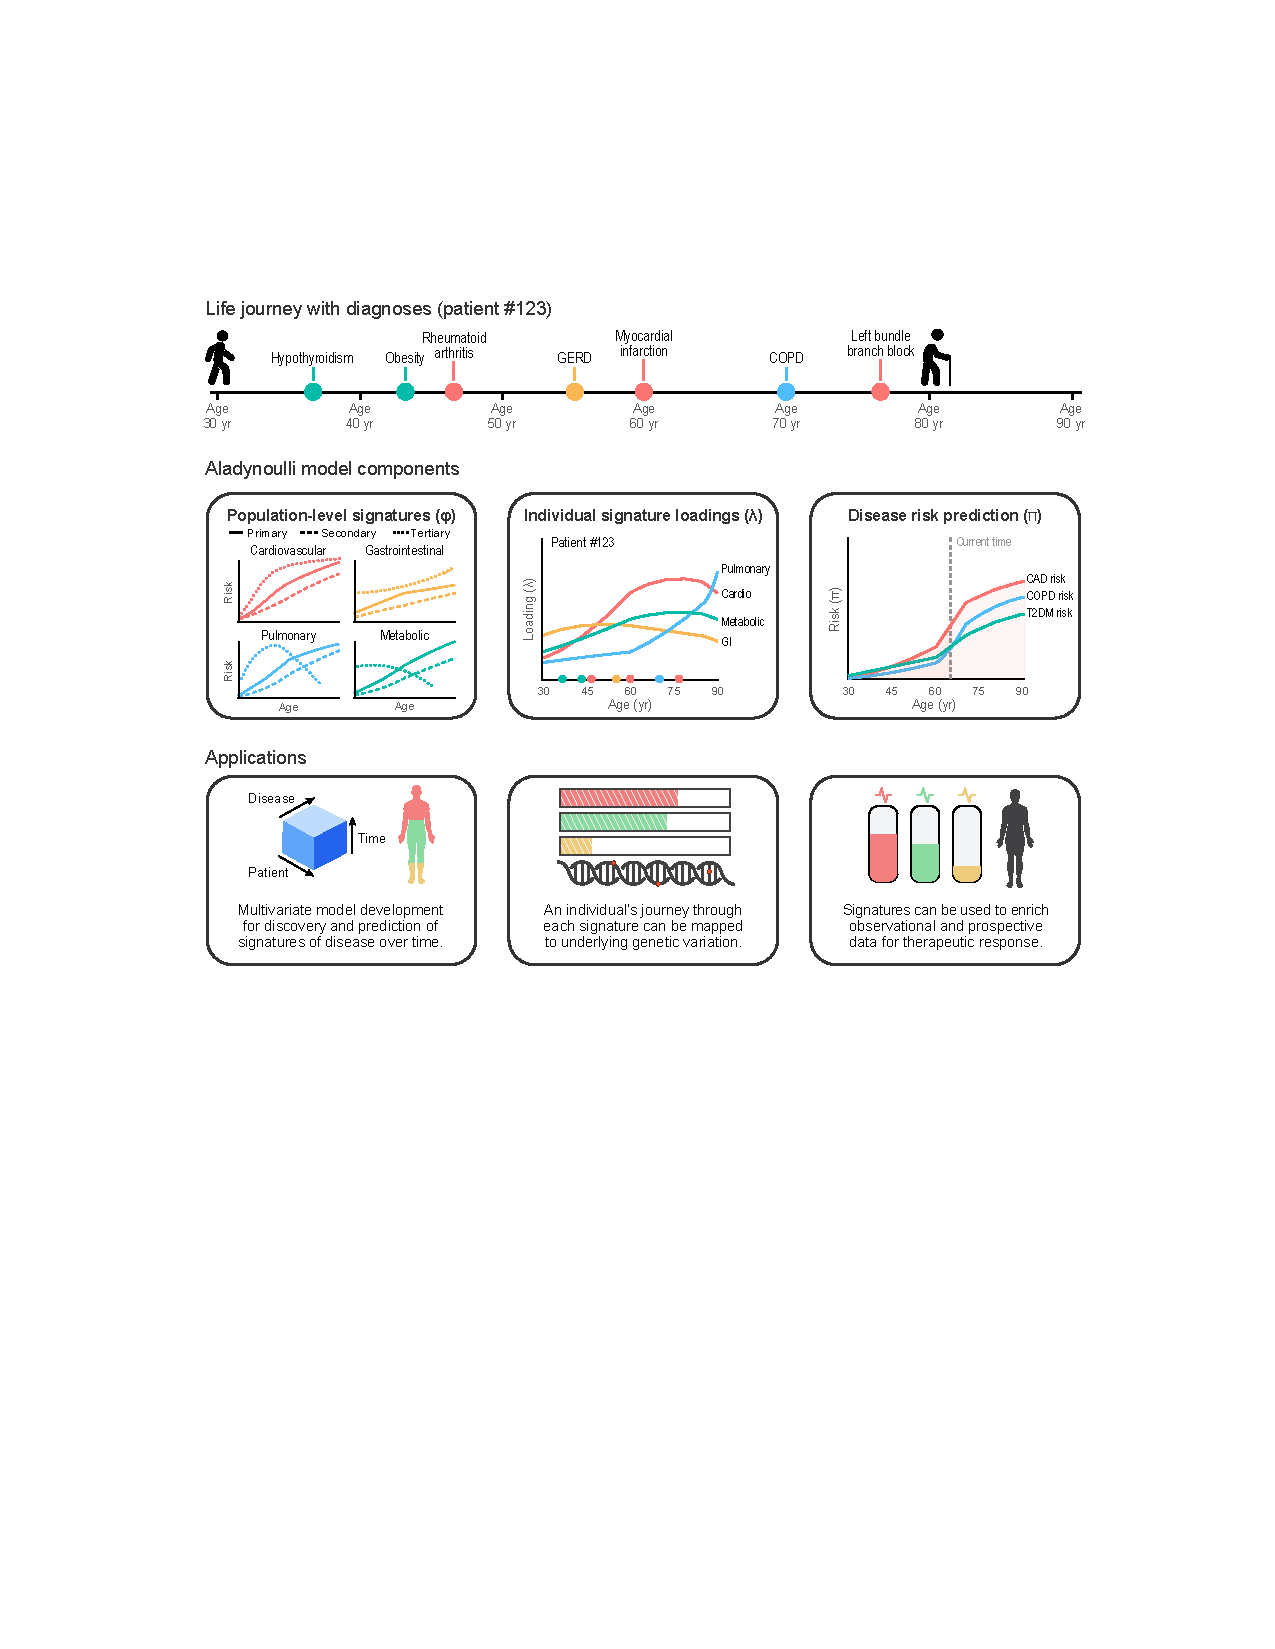
\includegraphics[width=1\textwidth]{alffigures/Fig1.pdf} % Model diagram
	% Pick an appropriate width
    \vspace*{12pt}
    \caption{\small{
        \textbf{\aladyn{} model overview and applications.}
        \textbf{Top:} Example patient timeline showing the sequence and timing of major diagnoses over the life course.
        \textbf{Middle:} Key model components. \textit{Left:} Population-level disease signatures ($\varphi$), with each line representing the age-dependent risk trajectory for a specific disease within a signature. \textit{Center:} Individual signature loadings ($\lambda$) transformed to $\theta$ via softmax, for a representative patient, showing how contributions from different signatures evolve over time. \textit{Right:} Disease risk prediction ($\pi$) for selected diseases, integrating population-level signatures and individual loadings to generate personalized risk trajectories.
        \textbf{Bottom:} Applications of the model, including genomic discovery, therapeutic targeting, and patient matching (e.g., digital twin identification or stratification of patients with the same diagnosis but different risk profiles).
        }}
        \label{fig:model_overview}
\end{figure}

\begin{figure} % Do NOT use \begin{figure*}
    \vspace*{-12pt}
\includegraphics[width=0.8\textwidth]{alffigures/Fig2.pdf} % Population-level
    \vspace*{12pt}

\caption{\small{\textbf{Population-level disease signatures inferred by \aladyn{}.}
(\textbf{A}) Age-dependent log hazard ratios for four representative disease signatures (cardiovascular, cancer, pulmonary, and cerebrovascular), as estimated by the model. Each line represents the predicted risk trajectory for a specific disease within the signature, illustrating distinct temporal patterns of disease onset.
(\textbf{B}) Heatmap of signature-disease specificity parameters $\hat{\psi}_{kd}$) learned by the model, with red indicating strong positive association and blue indicating negative association between diseases and signatures. (\textbf{C}) Cluster correspondence matrices comparing model-inferred disease groupings across biobanks (UK Biobank, MGB, and All of Us), demonstrating the consistency of disease clusters for common diseases.
(\textbf{D}) Model-predicted age-specific probabilities of disease onset for a range of conditions, showing the temporal emergence of diseases across the lifespan.
(\textbf{E}) Comparison of signature trajectories for cardiovascular and malignancy signatures across three independent biobanks (MGB, AoU, UKB), demonstrating the robustness and replicability of the model's temporal patterns across cohorts.
}}
\label{fig:signature-dynamics}
\end{figure}

\begin{figure}
    \vspace*{-12pt}
\includegraphics[width=0.85\textwidth]{alffigures/Fig3.pdf}
    \vspace*{12pt}
\caption{{\textbf{Individual-level trajectories and dynamic risk profiles.}
(A--C) Patient-specific normalized signature loadings ($\theta$) over time for three representative individuals. The lower panels show the disease timeline and key diagnoses for each patient.
(D) Comparison of early-onset ($<$55 years) and late-onset ($>$70 years) MI: Average signature loadings and their temporal velocities reveal distinct dynamic patterns and rates of change associated with age of onset.
(E) Decomposition of myocardial infarction (MI) risk for a representative patient: Top, time-varying signature loadings; middle, heatmap of log disease probabilities by signature and age; bottom, stacked area plot showing the aggregate risk over time.
(F) Signature heterogeneity within disease subtypes: Stacked area plots show deviations in signature proportions from the population average for selected diseases (malignant neoplasm of female breast, major depressive disorder, and myocardial infarction), highlighting the diversity of underlying biological processes among patients with the same clinical diagnosis.}}
\label{fig:individual_trajectories}
\end{figure}

\begin{figure}
\includegraphics[width=0.9\textwidth]{alffigures/Fig4.pdf}
    \vspace*{12pt}
\caption{\small{
\textbf{Genetic architecture and polygenic risk stratification of \aladyn{} disease signatures.}
(\textbf{A}) Top polygenic risk score (PRS) associations for each disease signature, showing effect sizes for the most significant PRS-signature pairs across disease categories.
(\textbf{B}) Heatmaps of mean PRS values by cluster for three representative diseases: major depressive disorder , breast cancer , and myocardial infarction , demonstrating the stratification of polygenic risk across model-inferred patient clusters.
(\textbf{C}) UpSet plot showing the overlap of genome-wide significant loci between disease signatures and individual traits, with analyses performed without PRS prior, highlighting shared genetic mechanisms across diseases. We consider SNPs as shared if they are within 1 MB of a lead loci in each componenet trait.
(\textbf{D}) Heatmap of positive genetic correlations ($r_g$) between disease signatures and complex traits, computed using LD score regression without PRS prior, revealing shared genetic architecture and pleiotropy.
}}
   \label{fig:genetics}
\end{figure}

\begin{figure}
    \centering
    \includegraphics[width=0.95\textwidth]{figures/signature_ancestry_lineplot.pdf}
    \caption{\textbf{Signature loadings show ancestry-specific temporal patterns that are amplified when genetic ancestry is explicitly modeled.} The figure displays signature-specific deviations from population reference across age (30-80 years) for four major ancestry groups: African (AFR), East Asian (EAS), South Asian (SAS), and European (EUR). Top row shows analyses without Principal Components (PCs); bottom row shows analyses with PCs included. Key findings: (1) \textbf{South Asian ancestry} shows strong enrichment in cardiovascular Signature 5 (light green), with deviation peaking around 0.025-0.03 at ages 50-60 when PCs are excluded, and dramatically amplified to 0.06 at age 60 when PCs are included, remaining elevated at 0.04 by age 80. This demonstrates that genetic ancestry substantially influences signature loadings and that explicitly modeling ancestry (via PCs) reveals stronger ancestry-specific patterns. (2) \textbf{East Asian ancestry} shows enrichment in Signature 8 (purple) and Signature 9 (brown), with patterns that become more pronounced when PCs are included. (3) \textbf{European ancestry} shows modest negative deviations in Signature 6 (red) at older ages. The temporal dimension reveals that ancestry effects on signatures evolve with age, with peak deviations occurring at different life stages for different ancestries. This analysis provides stronger evidence for biological validity than principal component associations alone because it demonstrates direct, interpretable relationships between ancestry and biologically meaningful disease signatures across the life course, rather than abstract statistical factors. The amplification of effects when PCs are included validates that genetic ancestry is a key determinant of signature loadings and should be explicitly modeled.}
    \label{fig:signature_ancestry}
\end{figure}

\begin{figure}
    \vspace*{-50pt}
    \includegraphics[width=0.9\textwidth]{alffigures/Fig5.pdf}
    \vspace*{12pt}
    \caption{\small
\textbf{Multi-Disease Risk Prediction Performance and Model Interpretation.}
(\textbf{A}) Discrimination performance across the top 16 diseases, measured by the area under the ROC curve (AUC) in a prospective, leakage-free framework. Each dot represents a different modeling approach. The primary approach, Median Aladynoulli 1-year (highlighted), reflects clinical practice: 1-year AUCs are computed for each year of follow-up using only data available up to that year, and the median AUC across years is reported. This represents how the model would be used in real-world clinical settings, making 1-year predictions at each patient visit. Aladynoulli Recruitment (1-year) uses predictions made at recruitment to evaluate 1-year outcomes, while Aladynoulli Recruitment (10-year) uses predictions made at recruitment to evaluate 10-year outcomes for comparison with clinical risk scores. PREVENT and PCE models are evaluated for their ability to predict 10-year outcomes using only recruitment data available at the time of study center visit. Cox models are fit using age as the time scale and include either Aladynoulli predictions, family history, and sex, or only family history and sex as covariates. All analyses exclude individuals with prevalent disease at time of prediction and use only information available up to the time of prediction, ensuring a fully prospective evaluation.
(\textbf{B}) Calibration plot across all follow-up periods for all at-risk individuals, showing observed versus predicted event rates on a log-log scale. Each point represents a bin of predicted risk, annotated with sample size; summary statistics (MSE, mean predicted, mean observed, total $N$) are provided.
(\textbf{C}) Model 10-year risk predictions versus incidence-based risk for ASCVD, stratified by age and percentiles. Solid lines show model-predicted mean and percentiles; the dashed line shows prevalence-based risk. $R^2$ indicates the correlation between predicted and observed risk.
(\textbf{D}) ROC curves for each year of the 10-year ASCVD prediction horizon, comparing the Aladynoulli model (AUC = 0.90), the PREVENT model (AUC = 0.649), and the Pooled Cohort Equations (PCE, AUC = 0.664).
(\textbf{E}) Softmax trajectory patterns for the latent patient loadings ($\lambda$): the upper panel shows individual patient trajectories for myocardial infarction (MI), censored prior to event; the lower panel shows mean trajectories for MI cases and controls, illustrating dynamic risk evolution over age.
}
    \label{fig:performance}
\end{figure}


%%%%%%%%%%%%%%%% REFERENCES %%%%%%%%%%%%%%%

\clearpage % Clear all remaining figures and tables then start a new page

% The list of references goes after the main text and before the acknowledgements
% When preparing an initial submission, we recommend you use BibTeX, like this:
%
%\include{suppclean}
\bibliography{exportforoverleaf,gprefs} % for a file named science_template.bib
\bibliographystyle{sciencemag}

% After the paper has completed peer review and been revised ready for acceptance,
% you should comment out the lines above and copy-paste the contents of your .bbl
% file here instead. This will help ensure that our conversion software works correctly.

%%%%%%%%%%%%%%%% ACKNOWLEDGEMENTS %%%%%%%%%%%%%%%

\section*{Acknowledgments}
\paragraph*{Funding:}
This work was supported by National Institutes of Health grants (R01HL155915, R01HL157635, R35HL144758) to P.N., American Heart Association grants (19SFRN34800000, 19SFRN34850009) to P.N.
\paragraph*{Author contributions:}
S.M.U., P.N. and G.P. conceptualized the study, developed the methodology, implemented the software, and wrote the original draft. Y.D. and X.J. contributed to methodology development and formal analysis. W.H. assisted with data curation and visualization. A.G., P.N., and G.P. provided supervision, resources, and critical review. All authors contributed to manuscript review and editing.
\paragraph*{Competing interests:}
The authors declare no competing interests.
\paragraph*{Data and materials availability:}
The code for implementing $\aladyn$ is available at https://github.com/surbut/aladynoulli2, with all analyses and code necessary for reproduction avaialable upon request from the authors.
Access to individual-level UK Biobank data requires approval from the UK Biobank (https://www.ukbiobank.ac.uk/). Access to Mass General Brigham data requires approval from the Mass General Brigham Institutional Review Board. Access to All of Us data requires approval through the All of Us Researcher Workbench (https://www.researchallofus.org/).




%%%%%%%%%%%%%%%% SUPPLEMENT TITLE PAGE %%%%%%%%%%%%%%%


%%%%%%%%%%%%%%%% SUPPLEMENT LIST %%%%%%%%%%%%%%%

% List the contents of your Extended Materials, including the numbers of any
% Extended figures, tables, external data files etc. and any references that are
% cited only in the supplement. In this example, refs. 7-8 are cited only in the supplement.
% Fill out your numbers accordingly and delete any lines that aren't applicable.


%%%%%%%%%%%%%%%% END OF MAIN TEXT %%%%%%%%%%%%%%%

\newpage

\renewcommand{\thefigure}{S\arabic{figure}}
\renewcommand{\thetable}{S\arabic{table}}
\renewcommand{\theequation}{S\arabic{equation}}
\renewcommand{\thepage}{S\arabic{page}}
\setcounter{figure}{0}
\setcounter{table}{0}
\setcounter{equation}{0}

\newpage

%%%%%%%%%%%%%%%% START OF SUPPLEMENT %%%%%%%%%%%%%%%
% Remove the duplicate commands that are currently here

\setcounter{page}{1}

%%%%%%%%%%%%%%%% SUPPLEMENT TITLE PAGE %%%%%%%%%%%%%%%



\section*{Extended Data for\\ \scititle}

\subsubsection*{This PDF file includes:}
Extended Data Figure S1 to S28\\
Extended Data Tables S1 to S9\\


\subsubsection*{Extended Data Files}
\begin{itemize}
  \item \textbf{Data S0:} PRS-signature association statistics (CSV; see \texttt{gamma\_associations.csv})
  \item \textbf{Data S1:} Cohen's d and p-values for signature differences between clusters in major depressive disorder (CSV)
  \item \textbf{Data S2:} Cohen's d and p-values for signature differences between clusters in breast cancer (CSV)
  \item \textbf{Data S3:} Cohen's d and p-values for signature differences between clusters in myocardial infarction (CSV)
  \item \textbf{Data S4:} Cohen's d and p-values for PRS differences between clusters in major depressive disorder (CSV)
  \item \textbf{Data S5:} Cohen's d and p-values for PRS differences between clusters in breast cancer (CSV)
  \item \textbf{Data S6:} Cohen's d and p-values for PRS differences between clusters in myocardial infarction (CSV)
  \item \textbf{Data S7-27:} Lead SNPs for each disease signature (TXT; one file per signature, including SNP ID, position, effect size, p-value, and annotation)
  \item \textbf{Data S28:} Pathway analysis for myocardial infarction heterogeneity (PDF; comprehensive pathway discovery analysis using deviation-from-reference clustering, showing four distinct biological pathways to MI with signature patterns, disease associations, genetic risk profiles, and cross-cohort validation between UK Biobank and Mass General Brigham)
\end{itemize}

\newpage

%Supp Figures

\begin{figure}[htbp]
    \centering
    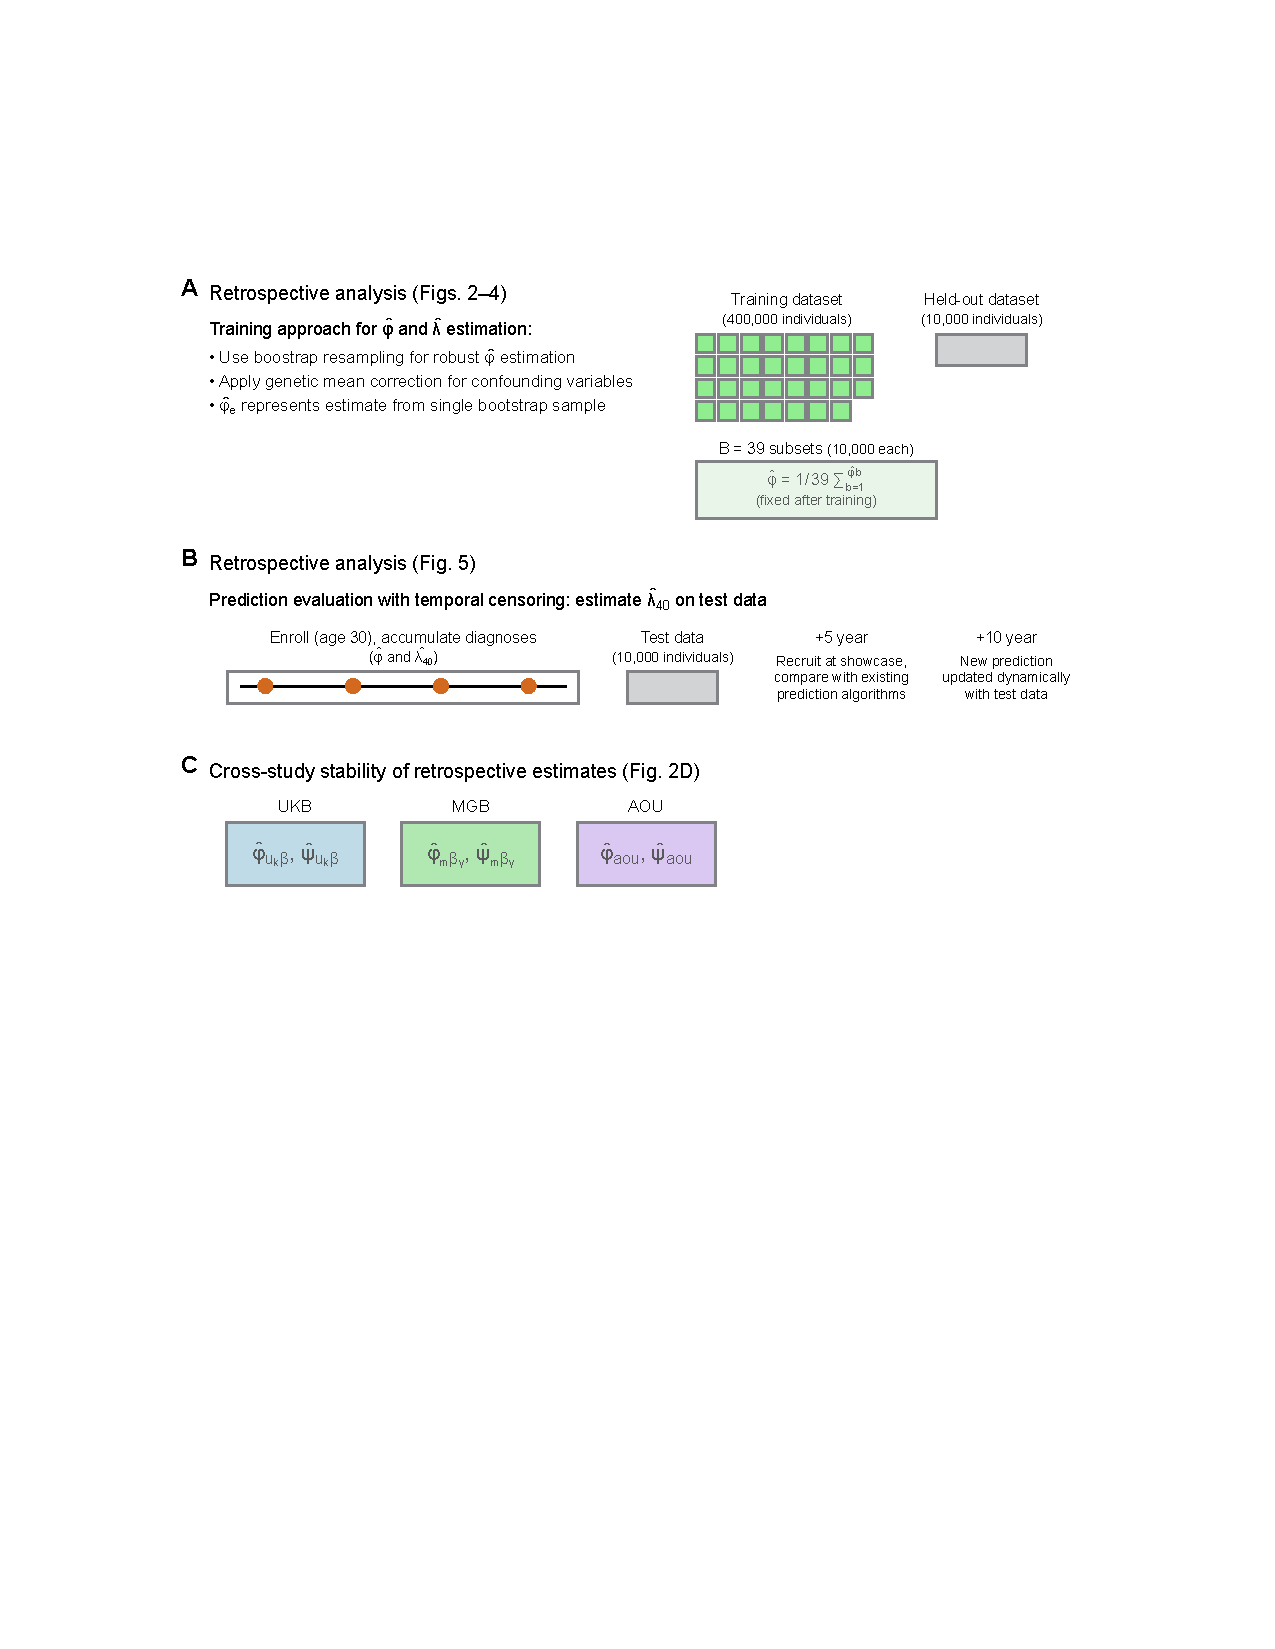
\includegraphics[width=0.95\textwidth]{alffigures/S3.pdf}
    \caption{\textbf{$\aladyn$} 
    (\textbf{A}) \textit{Retrospective Analysis (Figures 2-4):} UK Biobank training data (400k individuals) divided into 40 subsets of 10k each, with one subset held out for testing. Disease-signature associations ($\hat{\phi}$) and individual loadings ($\hat{\lambda}$) estimated on each of the 39 training subsets using complete disease trajectories, then averaged: $\phi_{\text{fixed train}} = \frac{1}{39} \sum_{b=1}^{39} \phi^{(b)}$. The held-out test set is never used for $\phi$ estimation, ensuring no data leakage. Genetic validation performed using models with genetic mean effects removed ($\Gamma_k = 0$).
    (\textbf{B}) \textit{Prospective Analysis (Figure 5):} Rigorous prediction evaluation using the held-out test set (10k individuals) with fixed $\phi_{\text{fixed train}}$ parameters. Individual loadings ($\hat{\lambda}_{\text{test}}$) re-estimated using only data available up to each prediction time point through temporal censoring. This approach prevents data leakage and simulates real-world clinical scenarios where population-level disease patterns are known but individual risk trajectories must be estimated prospectively from available clinical history.
    (\textbf{C}) \textit{Cross-Population Validation (Figure 2d):} Independent estimation of disease signatures in Mass General Brigham (MGB) and All of Us (AOU) cohorts demonstrates reproducibility across different populations and healthcare systems. Each cohort yields cohort-specific $\phi$ and $\psi$ parameters, with strong correlation between cohorts confirming biological validity rather than population-specific artifacts. This cross-population validation strengthens confidence in the universal applicability of discovered disease signatures.}
    \label{fig:training_architecture}
\end{figure}

\begin{figure}[htbp]

    \centering
    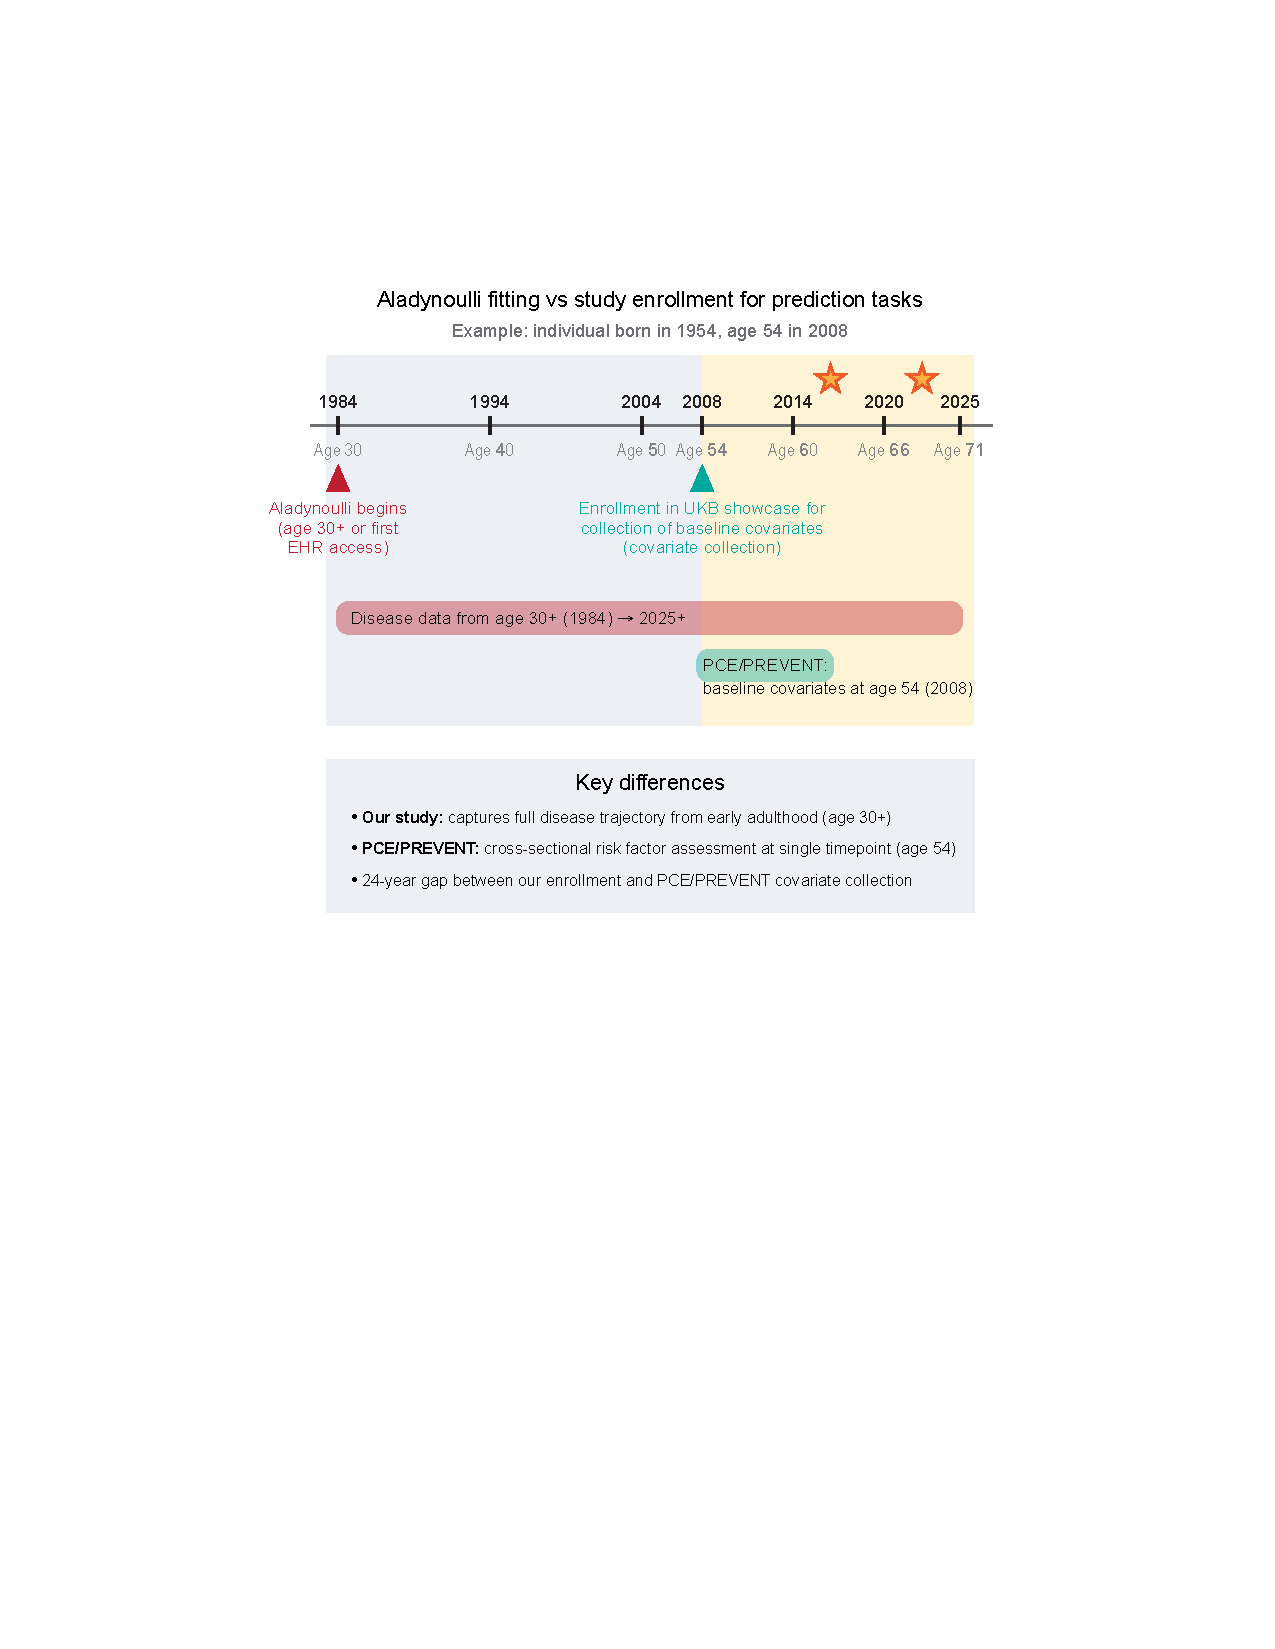
\includegraphics[width=0.8\linewidth]{alffigures/S9.pdf}
    \caption{\textbf{Enrollment Timeline} Schematic illustrating the distinction between the Aladynoulli model's use of longitudinal disease history (red) and the cross-sectional covariate collection at study recruitment (green) for risk prediction tasks. In this example, an individual's disease trajectory is captured from age 30 (or first EHR access) onward, enabling the Aladynoulli model to leverage decades of prior health data. In contrast, PCE and PREVENT models (\textbf{\ref{fig:roc_prevent}} use only baseline covariates collected at recruitment (age 54 in 2008). Outcome assessment is performed prospectively after recruitment (stars). The timeline highlights the 24-year gap between the start of disease data collection and the baseline covariate assessment, underscoring the unique ability of our approach to incorporate the full disease trajectory for prediction.}
    \label{fig:recruitment_timeline}
\end{figure}



\begin{figure}[htbp]
    \centering
    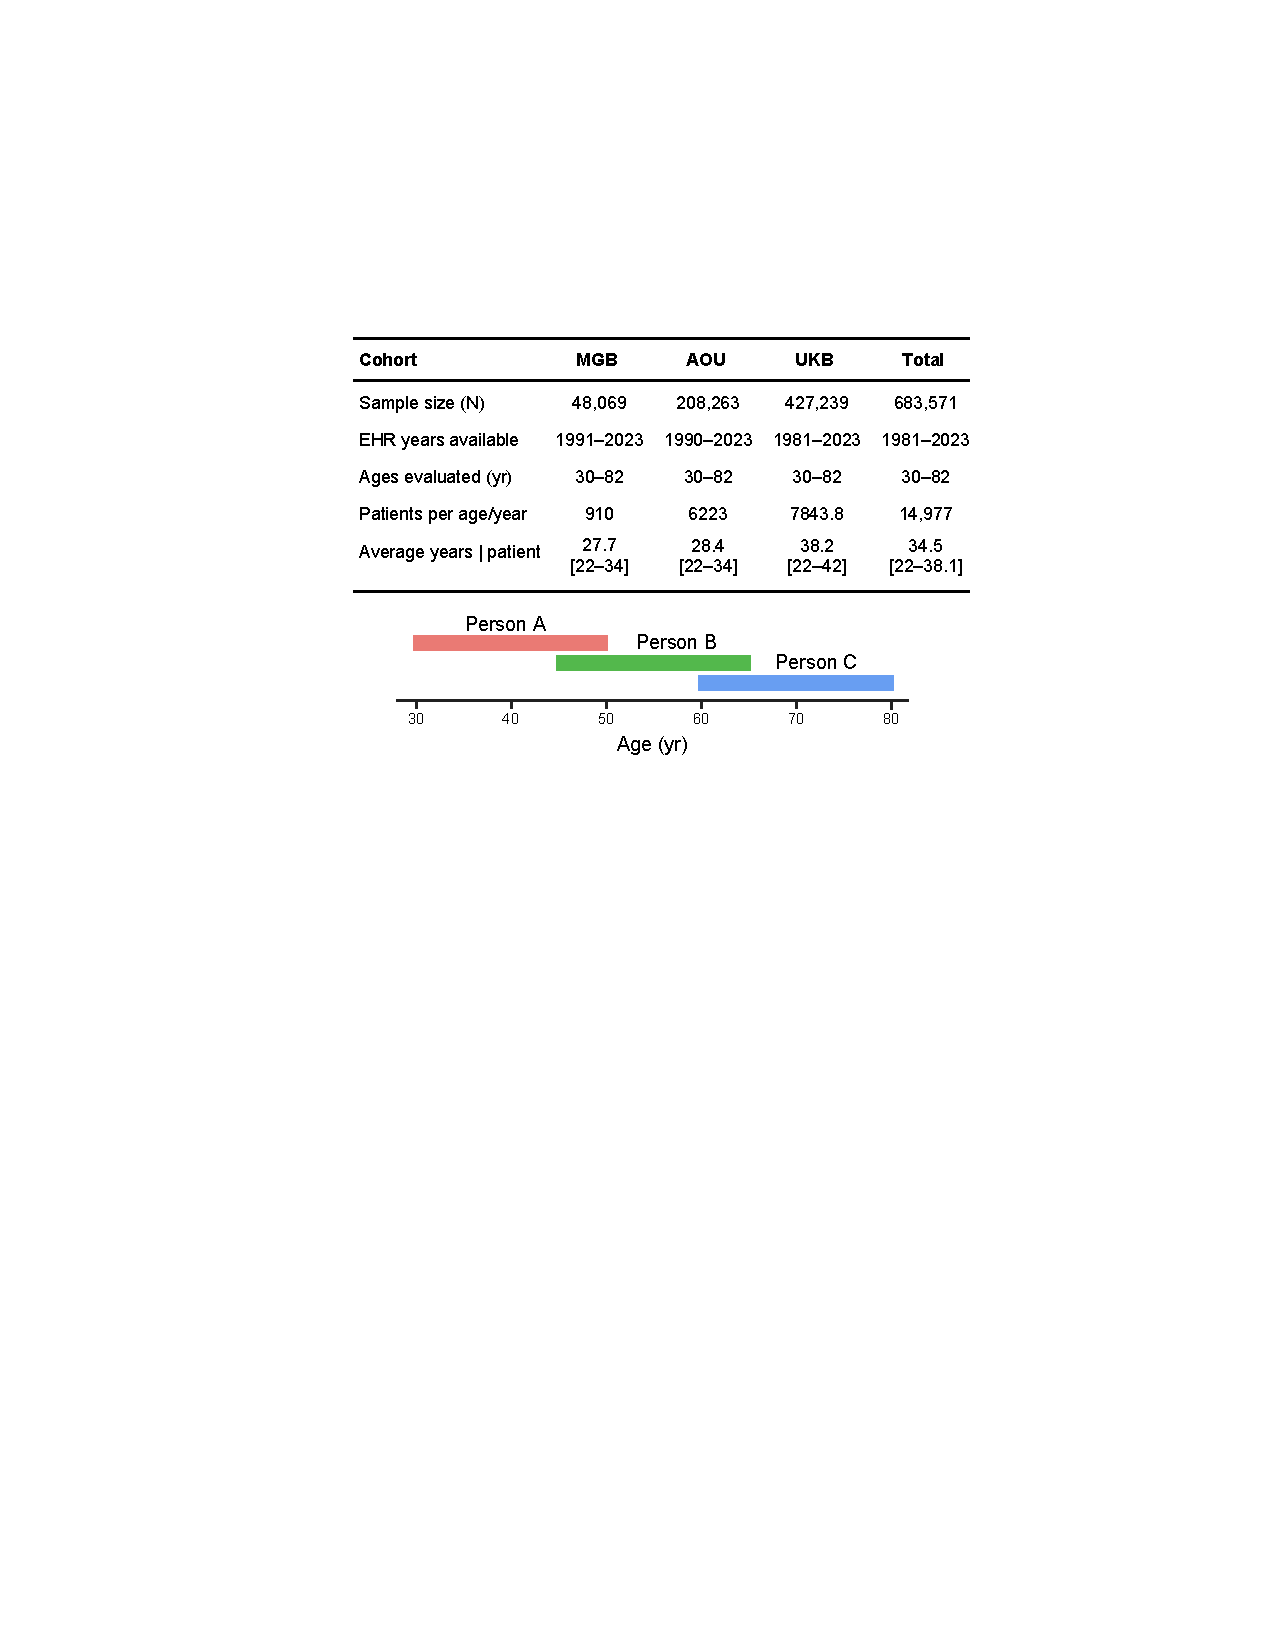
\includegraphics[width=0.9\linewidth]{alffigures/S13.pdf}
    \caption{\textbf{Cohort characteristics and study design.} Integration of partial life trajectories from three age groups (A: 30-50, B: 45-65, C: 60-82 years). The overlapping periods within each cohort enable robust estimation of disease trajectories across the full age spectrum.}
    \label{fig:cohort_design}
    \end{figure}
    

    
\begin{figure}[htbp]
    \centering
    \includegraphics[width=0.9\linewidth]{alffigures/S5.pdf}
    \caption{\textbf{Cross-cohort validation demonstrates robust disease signature replicability}. Heatmaps show the correspondence between \aladyn{} disease signatures (clusters) across cohorts, focusing on diseases common to all three biobanks. Each cell represents the proportion of diseases from a UK Biobank (UKB) signature that map to the corresponding signature in Mass General Brigham (MGB, left panel) or All of Us (AoU, right panel). Darker red indicates stronger correspondence. UKB clusters are ordered by their best-matching cluster in each validation cohort to highlight the diagonal pattern of correspondence. The analysis reveals high cross-cohort replicability, with a median maximum correspondence proportion of 0.792 across both validation cohorts, indicating that disease signatures identified in UK Biobank are consistently reproduced in independent healthcare systems.}
    \label{fig:cluster_correspondence}
\end{figure}



\begin{figure}[htbp]
\centering
\includegraphics[width=0.9\linewidth]{alffigures/S1.pdf}
\caption{\textbf{Robustness of $\phi$ estimation across subsets.} For each selected signature $k$ ($k=5,7,9,15,19$), we identified the disease $d$ with the highest $\psi_{k,d}$ in subset 1. For each $(k,d)$ pair, the plot shows the $\phi_{k,d}(t)$ trajectory over time for all subsets (gray lines), the mean across subsets (blue line), and the standard error (shaded region). The very small standard error demonstrates the stability of $\phi$ estimation across subsets.}
\label{fig:phi_batch}
\end{figure}


\begin{figure}[htbp]
    \centering
    \includegraphics[width=0.9\linewidth]{alffigures/S14.pdf}
\caption{\textbf{Temporal patterns of disease signatures across age in UK Biobank.} Each panel shows the probability trajectories for diseases within a signature across ages 30-81 years.}
\label{fig:temporal_ukb}
\end{figure}


\begin{figure}[htbp]
\centering
\includegraphics[width=0.9\linewidth]{alffigures/S15.pdf}
\caption{\textbf{Temporal patterns of disease signatures across age in All of Us.} Each panel shows the probability trajectories for diseases within a signature across ages 30-81 years.}
\label{fig:temporal_aou}
\end{figure}


\begin{figure}[htbp]
\centering
\includegraphics[width=0.9\linewidth]{alffigures/S16.pdf}
\caption{\textbf{Temporal patterns of disease signatures across age in MGB Biobank.} Each panel shows the probability trajectories for diseases within a signature across ages 30-81 years.}
\label{fig:temporal_mgb}
\end{figure}


\begin{figure}[htbp]
    \centering
    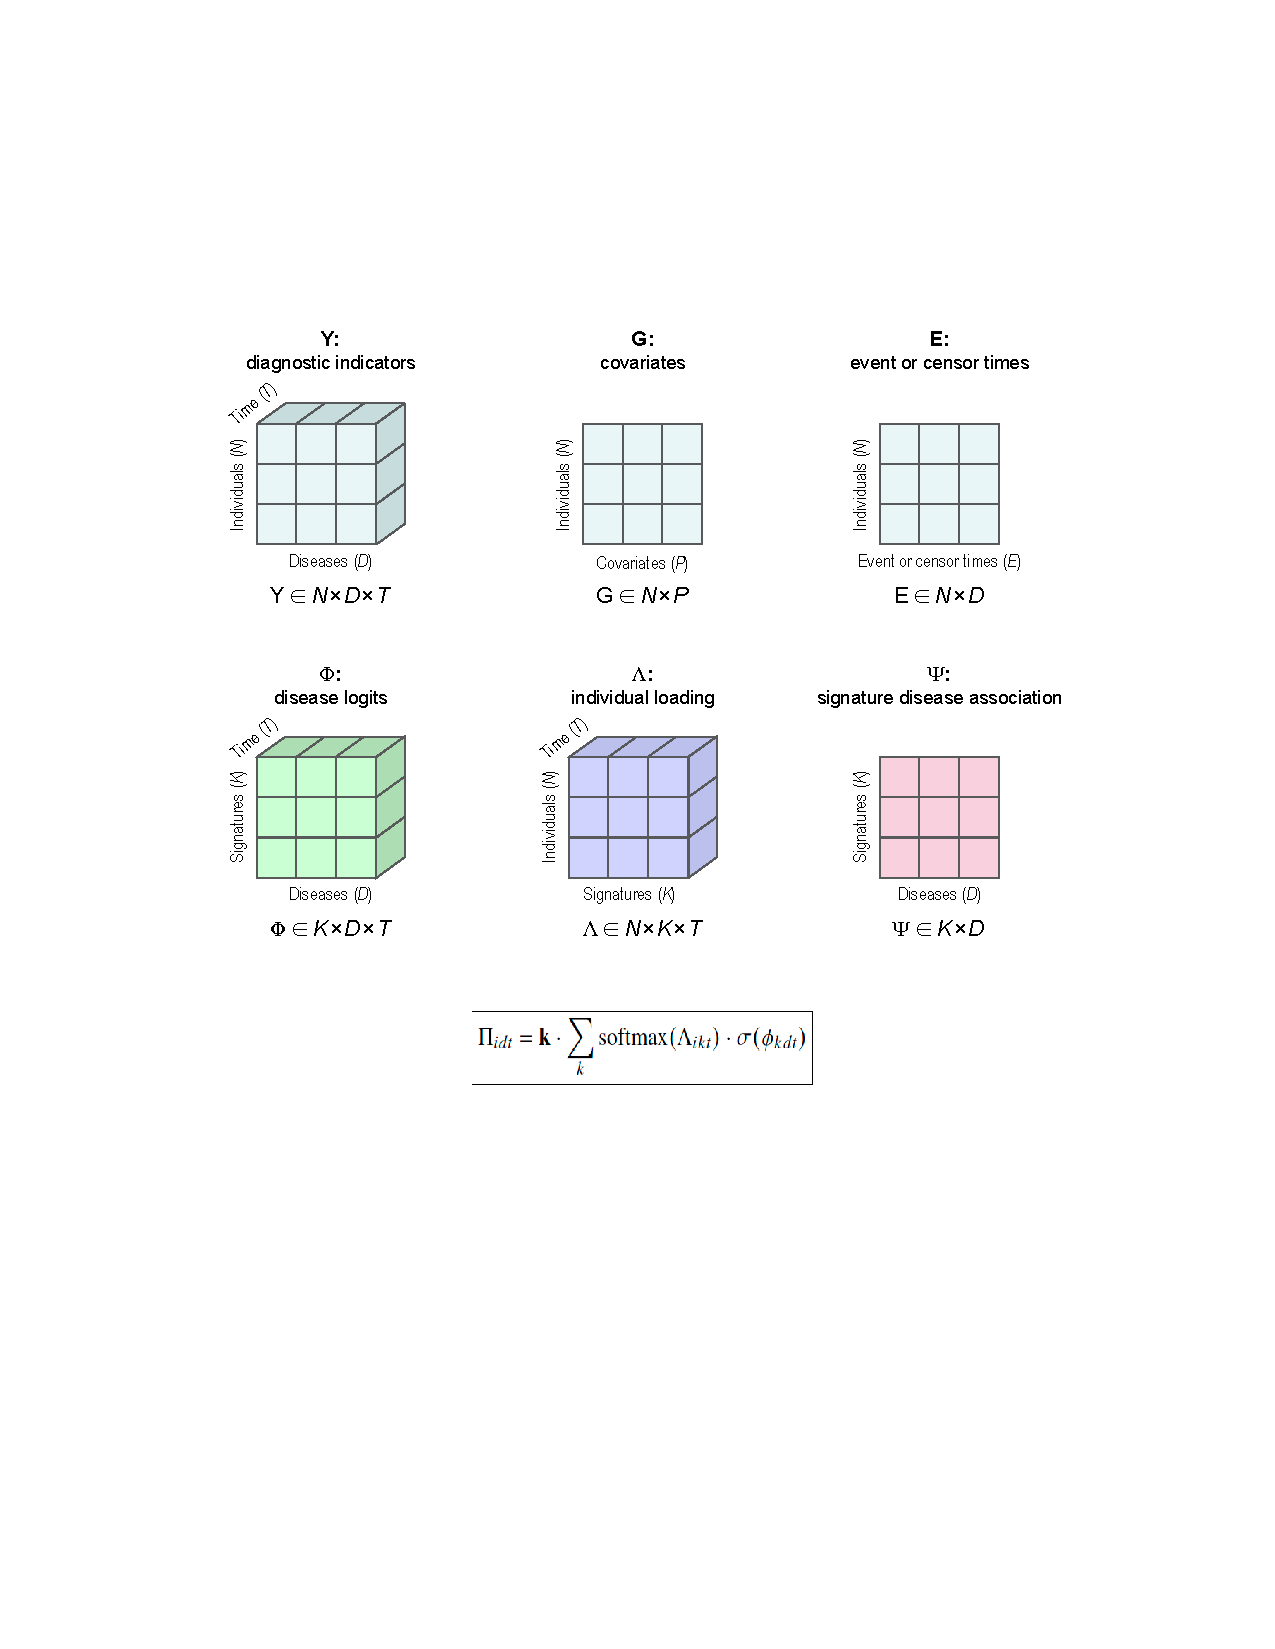
\includegraphics[width=0.75\linewidth]{alffigures/S12.pdf}
\caption{\textbf{\aladyn{} data structure and model components.} The figure illustrates the key data matrices and their relationships in the \aladyn{} framework. Top row: Input data includes Y (diagnostic indicators, a 3D tensor of binary disease outcomes across individuals, diseases, and time), G (covariates matrix for individuals), and E (event or censoring times). Bottom row: Model parameters include $\Phi$ (disease logits by signature and time), $\Lambda$ (individual loadings representing time-varying signature associations), and $\Psi$ (static signature-disease association strengths). The mathematical formula shows how these components combine to generate disease probabilities $\Pi_{idt}$ through a mixture of softmax-transformed individual loadings and sigmoid-transformed disease logits, scaled by a global calibration parameter.}
\label{fig:data-description}
\end{figure}



\begin{figure}[htbp]
    \centering
    \includegraphics[width=0.7\linewidth]{alffigures/S6.pdf}
    \caption{\textbf{Individual patient trajectories reveal distinct patterns of disease progression.}
    For each patient, the top panel shows normalized signature loadings ($\theta$) over time, with vertical dotted lines indicating disease diagnoses.
    The middle panel displays a chronological timeline of diagnosed conditions, with colors matching their primary signatures.
    The right panel shows the time-averaged signature contributions.
    Patients are ordered by increasing complexity of their disease profiles, from a single signature (top) to multiple interacting signatures (bottom).
    Colors are consistent across panels and represent the primary signature of each diagnosed condition.}
    \label{fig:patient_trajectories}
    \end{figure}

    

\begin{figure}[htbp]
    \centering
    \includegraphics[width=0.9\linewidth]{alffigures/S17.pdf}
    \caption{\textbf{Signature-based patient stratification reveals biological heterogeneity within clinical diagnoses.} Cohen's d effect sizes measuring the separation of time-averaged signature loadings between patient clusters for three representative diseases. Each bar represents the standardized difference in mean signature exposure between patients within a cluster versus those outside the cluster. Large positive values $(d \geq 0.8)$ indicate strong enrichment of a signature within that patient subgroup, while negative values indicate depletion. This analysis reveals distinct biological subtypes within traditional diagnostic categories, with different disease signatures showing varying degrees of patient stratification across clusters.}
    \label{fig:cohen_d}
    \end{figure}

    

    \begin{figure}[htbp]
        \centering
        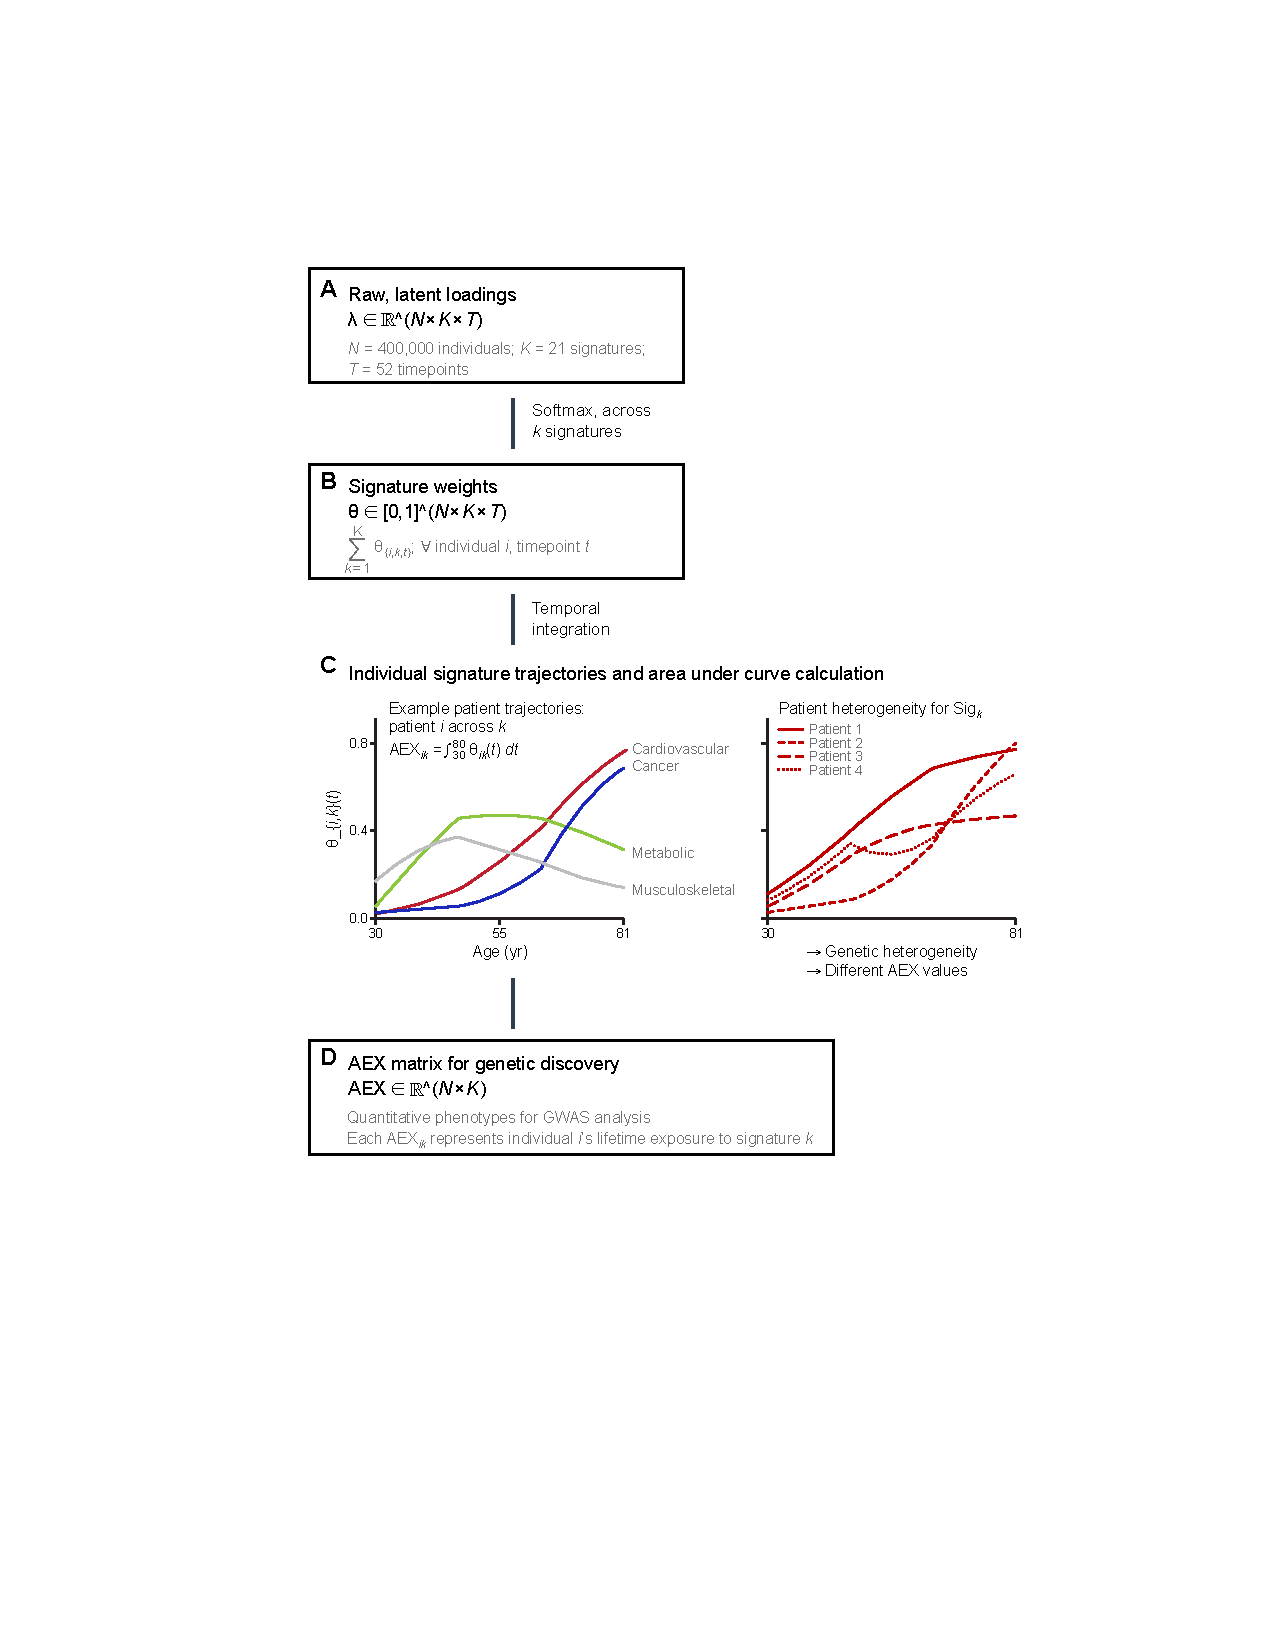
\includegraphics[width=0.9\textwidth]{alffigures/S4.pdf}
        \caption{\textbf{Average Exposure over time (AEX) calculation for genetic discovery.} 
        (\textbf{A}) \textit{Raw Latent Loadings:} The model estimates individual-specific  loadings $\hat{\lambda} \in \mathbb{R}^{N \times K \times T}$ for N=400,000 individuals across K=21 signatures and T=52 timepoints (ages 30-81). 
        (\textbf{B}) \textit{Signature Weights:} Raw loadings are transformed via softmax to obtain normalized signature loadings $\theta \in [0,1]^{N \times K \times T}$, where $\sum_k \theta_{i,k}(t) = 1$ for each individual and timepoint, representing the probability distribution across signatures.
        (\textbf{C}) \textit{Individual Signature Trajectories:} Left panel shows example temporal trajectories for different signatures (cardiovascular, cancer, metabolic, musculoskeletal) illustrating distinct age-related patterns. Right panel demonstrates patient heterogeneity within a single signature, showing how genetic and environmental factors lead to different AEX values across individuals.
        (\textbf{D}) \textit{AEX Matrix:} The area under each individual's signature trajectory is computed as $\text{AEX}_{i,k} = \int_{30}^{80} \theta_{i,k}(t) \, dt$, yielding a quantitative phenotype matrix $\text{AEX} \in \mathbb{R}^{N \times K}$ where each entry represents individual $i$'s lifetime exposure to signature $k$. This matrix serves as the input for genome-wide association studies to identify genetic variants influencing signature-specific disease risk patterns.}
        \label{fig:aex_calculation}
        \end{figure}





\begin{figure}[htbp]
    \centering
    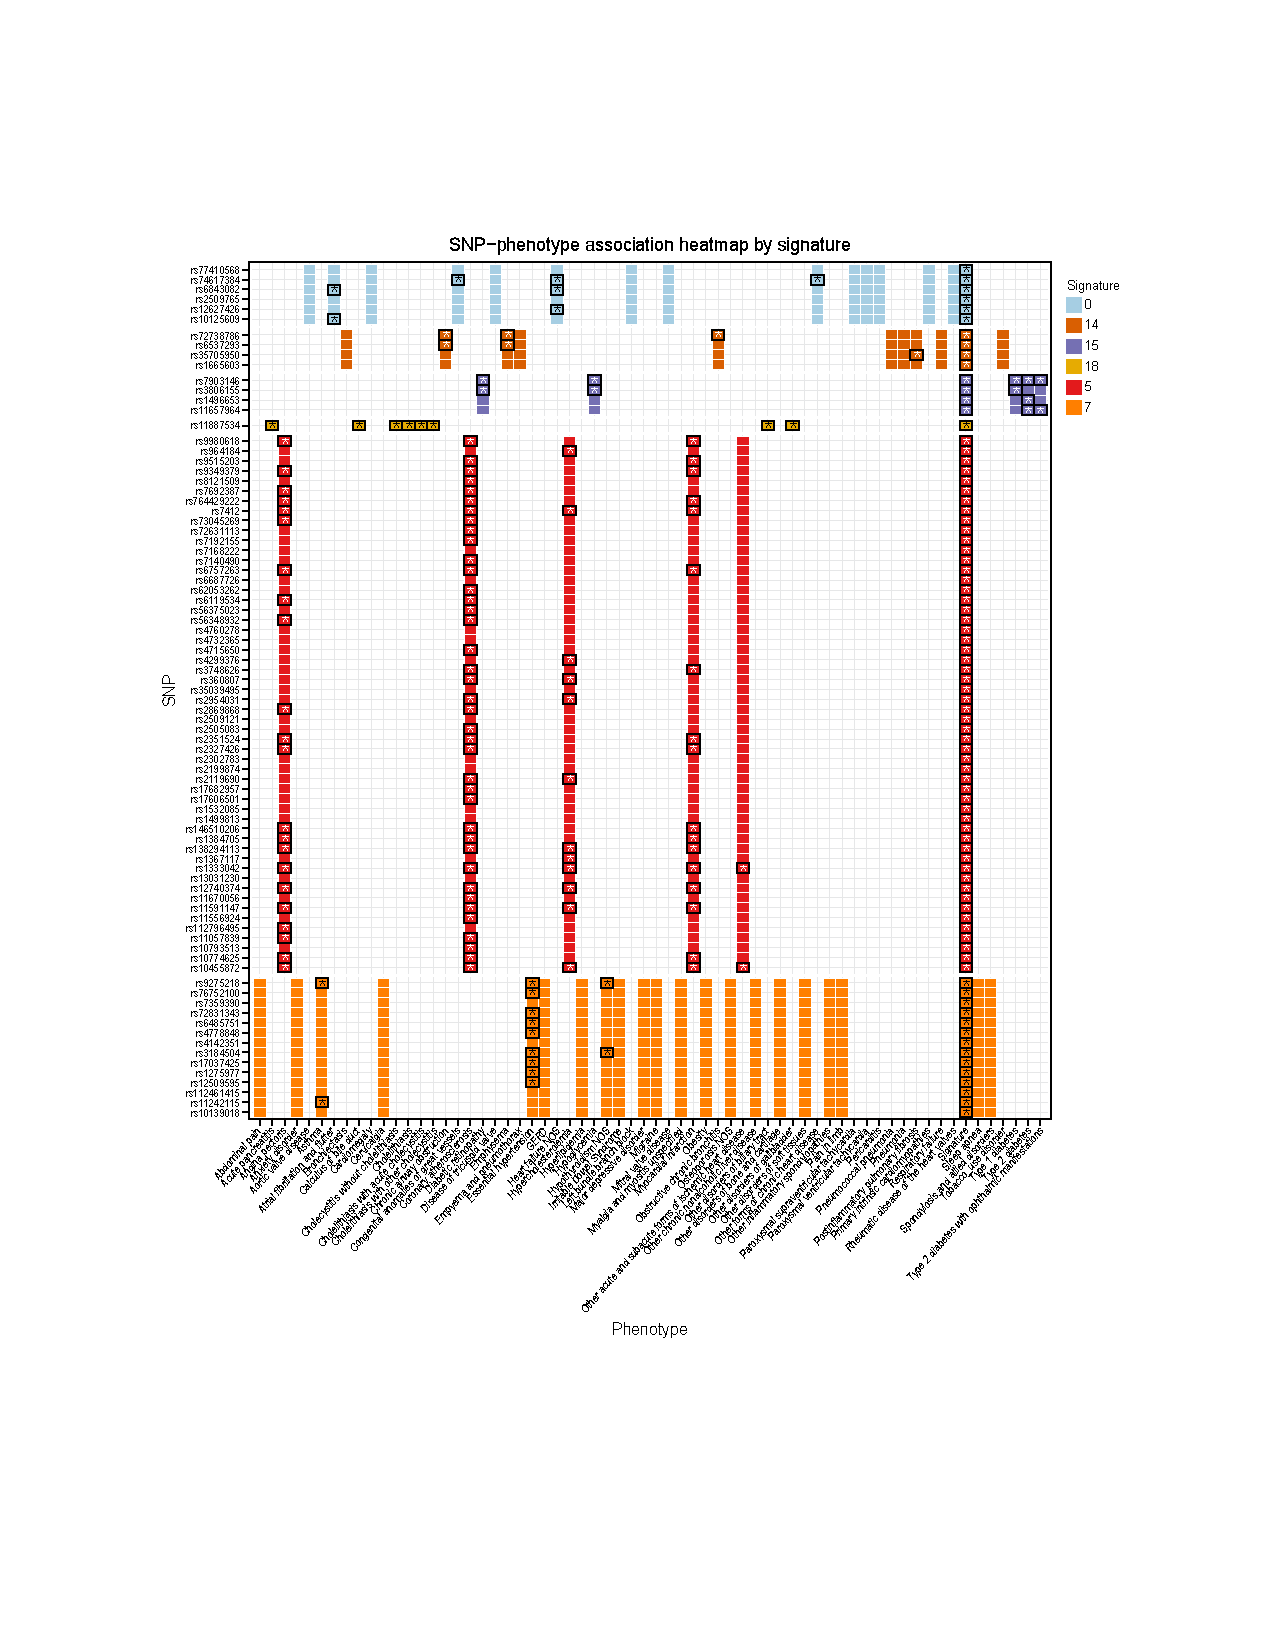
\includegraphics[width=0.9\linewidth]{alffigures/S7.pdf}
    \caption{\textbf{Signature-specific SNP associations reveal pleiotropic genetic effects.}
    For each \aladyn{} disease signature, we identified lead genetic variants (SNPs) from GWAS of the area-under-the-curve (AUC) of normalized signature loadings ($\theta$) across individuals. We then tested each lead SNP for association with a broad set of component disease phenotypes using logistic regression, adjusting for sex and ancestry principal components. The heatmap displays Z-statistics for the top signature-specific SNPs across all tested phenotypes, highlighting variants that are strongly associated with the signature trajectory but not with any single disease. These results reveal pleiotropic genetic effects that are captured by the multi-disease signature but are not apparent in single-disease GWAS.}
    \label{fig:snp_phenotype}
    \end{figure}
    

    \begin{figure}[htbp]
        \centering
        \includegraphics[width=0.7\linewidth]{alffigures/auc_trends_by_age.pdf}
        \caption{\textbf{Age-specific performance trends reveal substantial improvements from cumulative data inclusion.} AUC performance across 30 distinct prediction timepoints (ages 40-70 years) for diseases with sufficient events for reliable estimation ($\geq$ 3 years having $\geq$ 5 events). Each panel shows the evolution of predictive performance over age, with confidence intervals reflecting the precision of estimates at each timepoint. The cumulative data inclusion approach (using all available data from age 30 up to each prediction age) demonstrates remarkable performance improvements: ASCVD achieves median AUC of 0.985 across 28 years, Breast Cancer reaches 0.981 across 23 years, and Diabetes shows 0.948 across 25 years. This comprehensive evaluation across the adult lifespan reveals that the previous 10-year rolling window methodology significantly underestimated the model's true predictive capability, highlighting the importance of proper data inclusion strategies in survival prediction models.}
        \label{fig:auc_age}
        \end{figure}
    
        


    \begin{figure}[htbp]
        \centering
        \includegraphics[width=1.1\linewidth]{alffigures/S8.pdf}
        
        \caption{\textbf{ROC curves comparing \aladyn{} to PREVENT cardiovascular risk score.} Performance comparison for 10-year cardiovascular disease risk prediction using a the prediction at recruitment to predict 10 year outcomes in (\textbf{A}) the full population  (\textbf{B}) males only, and (\textbf{C}) females only. \aladyn{} demonstrates superior discrimination across all groups. This is not the optimal way to use \aladyn{} as we suggest dynamic updates (.e.g., calculated with new information at each stage) but we show here for comparability with the ASCVD which predicts for a 10-year horizon. Of note, the serious out performance of females versus males has been previously observed. \cite{ambrosio_performance_2025}}
        \label{fig:roc_prevent}
        \end{figure}
        
        
        

\begin{figure}[htbp]
    \centering
    \includegraphics[width=0.9\linewidth]{alffigures/S10.pdf}
    \caption{\textbf{Distribution of 1-year AUCs across offsets for each disease}
    Each violin shows the distribution of AUC values obtained from prospective, leakage-free 1-year risk predictions at different follow-up offsets for the indicated disease. Points within each violin represent the AUC at a specific offset. This visualization highlights both the variability and the central tendency of model discrimination performance over time for each disease.}
    \label{fig:1yearoffsetviolin}
    \end{figure}



\begin{figure}[htbp]
    \centering
    \includegraphics[width=0.9\linewidth]{alffigures/gail.png}
    \caption{\textbf{Evaluation of GAIL Model}
   AUC comparing the use of the GAIL score which incorporates female history, age at menses, and number of first degree relatives with breast cancer verus $\aladyn$ naiive trained model at recruitment on ten year outcomes.}
    \label{fig:gail}
    \end{figure}
    
    
    \newpage
    
    \begin{figure}[htbp]
    \centering
    \includegraphics[width=0.9\linewidth]{alffigures/S11.pdf}
    \caption{\textbf{Distribution of 1-year AUCs across offsets for ASCVD versus commonly used clinical risk scores}
    Receiver operating characteristic (ROC) curves for 1-year ASCVD risk prediction at each follow-up year, comparing the Aladynoulli model (solid lines), Pooled Cohort Equations (PCE, dashed lines), and PREVENT (dotted lines). For each offset (year since recruitment), the model's predicted 1-year risk is evaluated against observed 1-year outcomes, excluding individuals with prevalent ASCVD at the start of each interval. The area under the curve (AUC) for each method and year is shown in the legend. This visualization demonstrates the discrimination performance of each approach over time, highlighting the dynamic updating capability of Aladynoulli compared to static clinical risk scores.}
    \label{fig:one_year_vsPCE}
    \end{figure}


    
\begin{figure}[htbp]
\centering
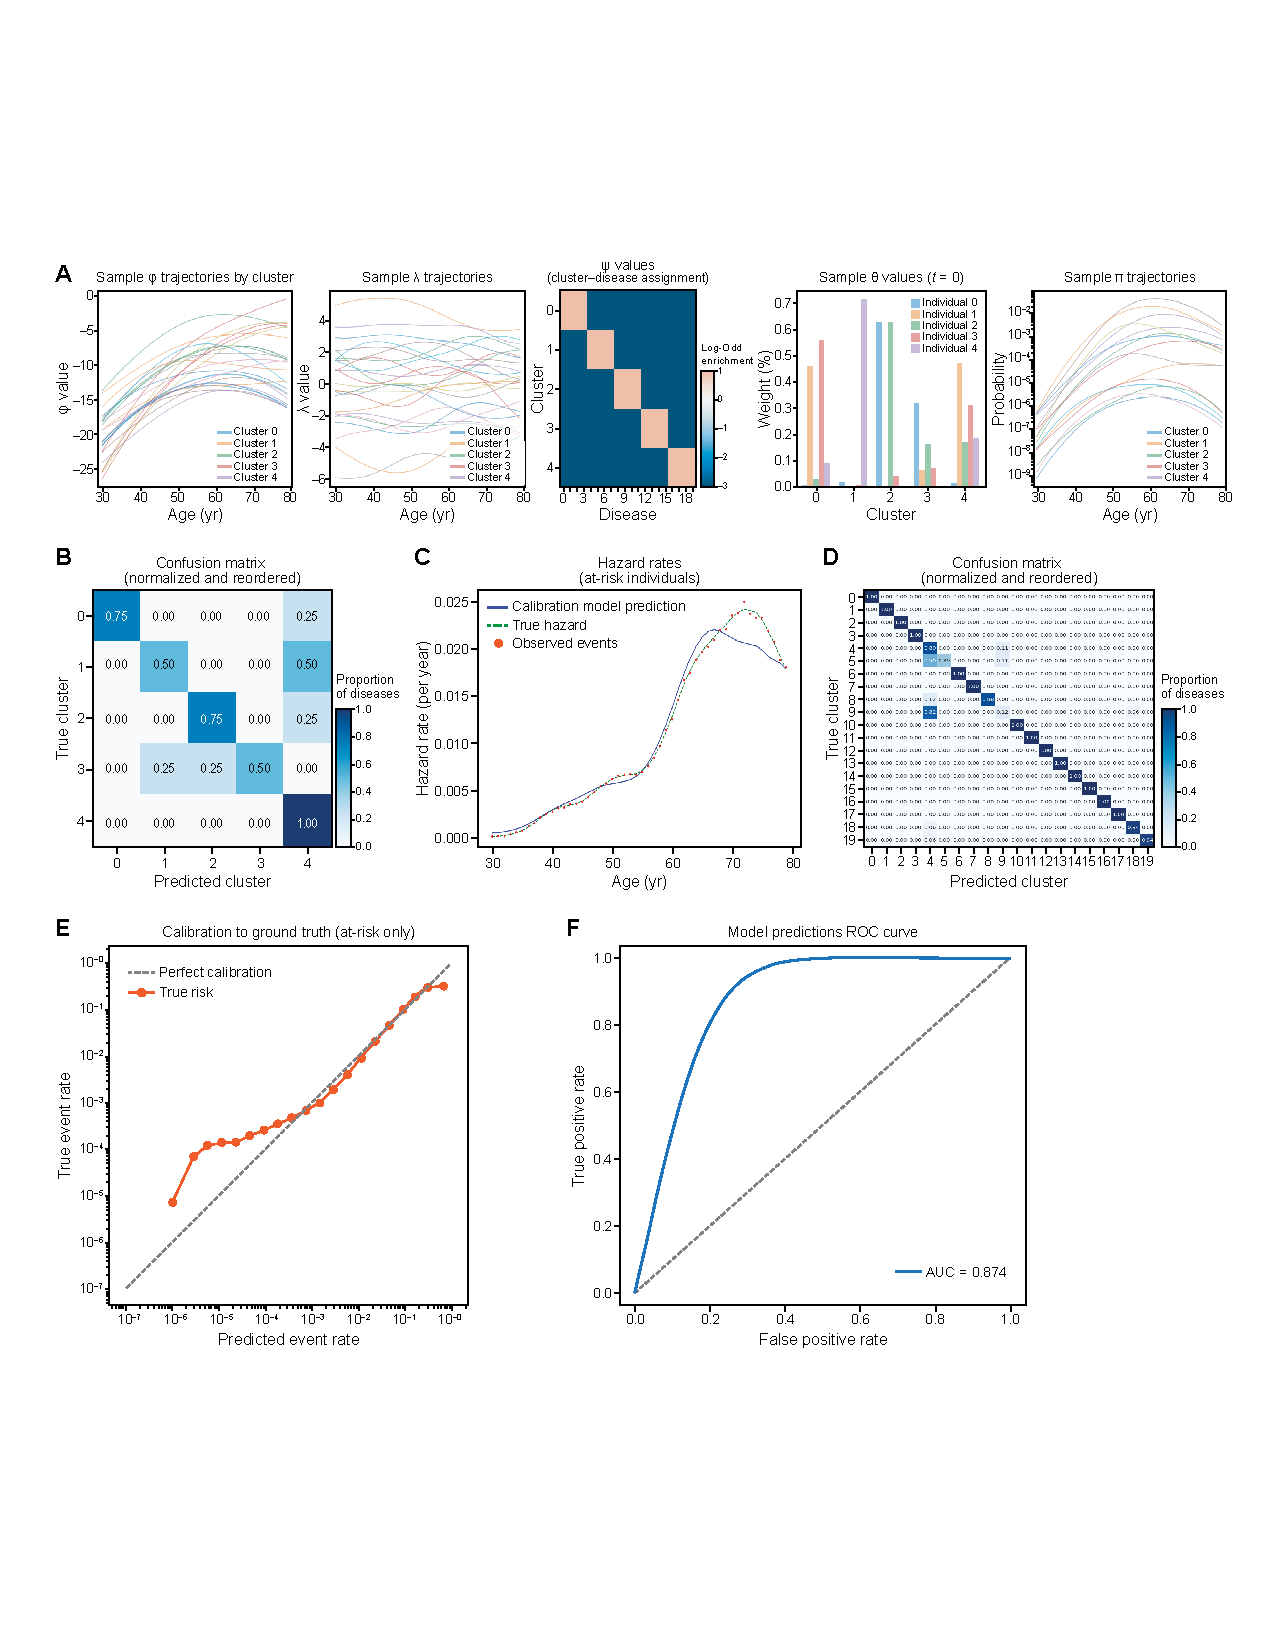
\includegraphics[width=0.9\linewidth]{alffigures/S2.pdf}

\caption{\textbf{Simulation study demonstrates accurate recovery of latent disease clusters and temporal dynamics.}
(\textbf{A}) Simulated disease baseline trajectories on the logit scale, showing diverse prevalence and onset patterns.
(\textbf{B}) Example latent signature trajectories for individual patients, illustrating temporal smoothness and genetic heterogeneity.
(\textbf{C}) True and inferred disease cluster assignments visualized as a confusion matrix.
(\textbf{D}) Correlation matrix comparing true and inferred cluster assignments.
(\textbf{E}) Comparison of true and model-inferred hazard rates over time.
(\textbf{F}) ROC curve for simulated disease prediction, demonstrating high discriminative performance.
Together, these results confirm that the \aladyn{} model can accurately recover both the cluster structure and temporal risk dynamics from complex, realistic simulated data.}
\label{fig:simulation}
\end{figure}


%\subsection*{Extended Tables}
%clearpage

\begin{table}
\singlespacing
\centering
\caption{\textbf{Notation and Dimensions.} Mathematical notation and parameter definitions used throughout the \aladyn{} model. The table organizes symbols by category (dimensions, data structures, model parameters, and hyperparameters) to provide a comprehensive reference for the model's mathematical framework. Each symbol is defined with its corresponding dimension, data type, and role in the model architecture.}
\label{tab:notation}
\begin{tabular}{llll}
\toprule
\textbf{Symbol} & \textbf{Description} & \textbf{Dimension} & \textbf{Type} \\
\midrule
\addlinespace
\multicolumn{4}{l}{\textit{Dimensions}} \\
$N$ & Number of individuals &  &  \\
$D$ & Number of diseases &  &  \\
$T$ & Number of time points &  &  \\
$K$ & Number of signatures &  &  \\
$P$ & Number of covariates &  &  \\
%
\multicolumn{4}{l}{\textit{Data}} \\
$\mathbf{Y}$ & Disease indicator tensor & $N \times D \times T$ & Binary \\
$\mathbf{g}_i$ & Covariate (genetic/demographic) vector for individual $i$ & $P$ & Real \\
$\mathbf{E}$ & Event/censoring time matrix & $N \times D$ & Integer \\
\addlinespace
\multicolumn{4}{l}{\textit{Model Parameters}} \\
$\boldsymbol{\Pi}$ & Disease probability tensor & $N \times D \times T$ & $[0,1]$ \\
$\boldsymbol{\Theta}$ & Normalized loadings (softmax of $\boldsymbol{\Lambda}$) & $N \times K \times T$ & $[0,1]$ \\
$\boldsymbol{\Lambda}$ & Latent signature loadings & $N \times K \times T$ & Real \\
$\boldsymbol{\Phi}$ & Disease-signature association & $K \times D \times T$ & Real \\
$\boldsymbol{\Psi}$ & Static signature-disease strength & $K \times D$ & Real \\
$\boldsymbol{\mu}_d$ & Disease baseline trajectory for disease $d$ & $T$ & Real \\
$\boldsymbol{\gamma}_k$ & Covariate effects for signature $k$ & $P$ & Real \\
$\kappa$ & Global calibration parameter & Scalar & $\mathbb{R}^+$ \\
\addlinespace
\multicolumn{4}{l}{\textit{Hyperparameters}} \\
$\alpha_\lambda$ & Amplitude for Gaussian Process on $\lambda$'s & Scalar & $\mathbb{R}^+$ \\
$l_\lambda$ & Length scale for Gaussian Process on $\lambda$'s & Scalar & $\mathbb{R}^+$ \\
$\alpha_\phi$ & Amplitude for Gaussian Process on $\phi$'s & Scalar & $\mathbb{R}^+$ \\
$l_\phi$ & Length scale for Gaussian Process on $\phi$'s & Scalar & $\mathbb{R}^+$ \\
$\sigma^2_\gamma$ & Variance of covariate effects & Scalar & $\mathbb{R}^+$ \\
\bottomrule
\end{tabular}
\end{table}




\begin{table}
    \singlespacing
    
    \caption{\textbf{Baseline characteristics vary across the three study cohorts.} The table presents demographic and clinical characteristics for each cohort (MGB, AoU, UKB), including recruitment age, sex distribution, genetic ancestry composition, and healthcare utilization patterns. Each column represents a different cohort, with values shown as mean (SD) for continuous variables and n (\%) for categorical variables. The genetic ancestry categories (EUR, AFR, AMR, EAS, SAS) reflect the population diversity across cohorts, while healthcare utilization metrics (number of diagnoses, median age at diagnosis) indicate differences in data availability and clinical patterns.}
    \label{tab:baseline_characteristics}
    \begin{tabular}{lccc}
    \toprule
    Variable & MGB (N=48,069) & AoU (N=208,263) & UKB (N=427,239) \\
    \midrule
    recruitment Age (years) & 54.3 (17.1) & 59.4 (14.3) & 57.2 (8.0) \\
    Female, n (\%) & 26,295 (55.4\%) & 128,082 (61.5\%) & 233,205 (54.6\%) \\
    \addlinespace
    \textit{Genetic Ancestry} & & & \\
    EUR & 32,811 (69.2\%) & 84,164 (40.4\%) & 387,119 (90.6\%) \\
    AFR & 2,113 (4.5\%) & 28,651 (13.7\%) & 7,158 (1.7\%) \\
    AMR & 2,785 (5.9\%) & 21,401 (10.3\%) & 607 (0.1\%) \\
    EAS & 770 (1.6\%) & 2,313 (1.1\%) & 1,715 (0.4\%) \\
    SAS & 425 (0.9\%) & 1,147 (0.6\%) & 7,915 (1.9\%) \\
    NA (Missing) & 8,524 (18.0\%) & 58,410 (28.0\%) & 22,727 (5.3\%) \\
    \addlinespace
    Number of Diagnoses, median [IQR] & 28.0 [38.0] & 18.0 [28.0] & 6.0 [9.0] \\
    Median Age at Diagnosis, median [IQR] & 58.0 [26.0] & 54.0 [22.0] & 63.3 [15.2] \\
    Ages Considered & 30--81 & 30--81 & 30--81 \\
    EHR Years Available & 1991--2023 & 1990--2023 & 1981--2023 \\
    Average number of patients per age-year bin & 910 & 6,223 & 7,843 \\
    \bottomrule
    \end{tabular}
    \end{table}


\begin{table}
\centering
\singlespacing
\caption{\textbf{Disease signatures identified by \aladyn{} show distinct clinical domains.} The table lists all 20 disease signatures discovered by the model, showing representative associated diseases with their odds ratios (OR) in parentheses, the total number of diseases in each signature, and the primary clinical domain. Each signature represents a distinct biological pathway or disease process, with diseases grouped based on their co-occurrence patterns and temporal dynamics. The odds ratios indicate the strength of association between each disease and its assigned signature.}
\label{tab:signature_summary_actual}
\footnotesize
\begin{tabular}{c p{7.5cm} p{3.5cm}}
\toprule
\textbf{Sig} & \textbf{Representative Associated Diseases (OR) [Total: N diseases]} & \textbf{Clinical Domain} \\
\midrule
0 & Atrial fibrillation (5.05), Heart failure (4.33), Cardiomegaly (3.58) [16] & Cardiac Arrhythmias \\
1 & Hallux valgus (3.60), Enthesopathy (3.57), Peripheral enthesopathies (3.52) [21] & Musculoskeletal \\
2 & Diaphragmatic hernia (4.29), Gastritis (3.94), GERD (3.91) [15] & Upper GI/Esophageal \\
3 & Peripheral vascular disease (3.12), Right bundle branch block (3.03), Other tests (3.12) [82] & Mixed/General Medical \\
4 & Upper respiratory disease (3.00), Septal deviations (2.69), Nasal polyps (2.64) [5] & Upper Respiratory \\
5 & Coronary atherosclerosis (4.97), Hypercholesterolemia (4.79), Angina (4.57) [7] & Ischemic cardiovascular \\
6 & Secondary lymph malignancy (4.05), Secondary liver malignancy (3.69), Lung cancer (3.26) [8] & Metastatic Cancer \\
7 & Myalgia (2.82), Rheumatism/fibrositis (2.57), Cervicalgia (2.48) [22] & Pain/Inflammation \\
8 & Uterine polyp (3.69), Cervicitis (3.62), Uterine prolapse (3.59) [28] & Gynecologic \\
9 & Back pain (6.83), Spondylosis (4.60), Radiculitis (4.25) [12] & Spinal Disorders \\
10 & Cataract (4.56), Senile cataract (4.52), Macular degeneration (4.46) [11] & Ophthalmologic \\
11 & Cerebral artery occlusion (3.86), Cerebral infarction (3.36), Cerebral ischemia (3.36) [8] & Cerebrovascular \\
12 & Renal colic (3.62), Hydronephrosis (3.07), Ureter obstruction (2.88) [7] & Renal/Urologic \\
13 & Prostate cancer (5.96), Prostate hyperplasia (5.47), Urethral stricture (4.66) [13] & Male Urogenital \\
14 & Tobacco use disorder (4.55), Chronic airway obstruction (3.87), Pneumonia (3.77) [10] & Pulmonary/Smoking \\
15 & Type 2 diabetes (6.40), Hypoglycemia (3.83), Diabetic eye disease (3.53) [5] & Metabolic/Diabetes \\
16 & Other anemias (3.30), Acute renal failure (3.10), E. coli (3.13) [29] & Infectious/Critical Care \\
17 & Colon neoplasm (3.77), Diverticulosis (3.64), Hemorrhoids (3.50) [17] & Lower GI/Colon \\
18 & Cholelithiasis (4.57), Peritoneal adhesions (4.21), Gallbladder disorders (4.03) [9] & Hepatobiliary \\
19 & Skin cancer (4.82), Benign skin neoplasm (3.90), Actinic keratosis (3.84) [23] & Dermatologic/Oncologic \\
\bottomrule
\end{tabular}
\end{table}





\begin{table}[t]
\centering
\singlespacing
\caption{\textbf{Prediction methodologies differ in their temporal approach and data usage.} The table defines five distinct prediction approaches used to evaluate \aladyn{} performance, and additionally includes the rolling interpolation. Each method is described in terms of its temporal updating strategy, data availability constraints, and evaluation framework. The methods progress from most sophisticated (dynamic updating with temporal censoring) to baseline comparisons (traditional Cox models without \aladyn{} features), providing a comprehensive evaluation of the model's predictive capabilities across different clinical scenarios.}
\begin{tabular}{|p{3cm}|p{10cm}|}
\hline
\textbf{Method} & \textbf{Definition} \\
\hline
Median Aladynoulli 1-year & Dynamic 1-year risk predictions using models trained with data available up to each prediction time point, evaluated over 1-year windows. Median AUC across rolling one-year predictions is reported. \\
\hline
Aladynoulli 1-year & 1-year risk prediction made at cohort recruitment time using model trained on data available up to recruitment . Single prediction evaluated against 1-year outcomes. \\
\hline  

Rolling Aladynoulli 10-year & Cumulative 10-year risk calculated as the product of yearly survival probabilities: $1 - \prod_{t=1}^{10}(1 - \pi_t)$ where each $\pi_t$ comes from the rolling 1-year predictions above. \\
\hline
Aladynoulli 10-year & 10-year risk prediction using single model trained only on data available at recruitment, without any temporal updating during follow-up, evaluated on 10 year outcomes. \\
\hline
Cox with Aladynoulli & Cox proportional hazards model including traditional predictors (age, sex, family history) plus baseline Aladynoulli risk prediction at recruitment (on model fit using using data up until prediction time) as covariates. \\
\hline
Cox without Aladynoulli & Cox proportional hazards model using only traditional predictors (age, sex, family history when available). Baseline comparison model. \\
\hline
\end{tabular}

\label{tab:prediction_methods}
\end{table}




\begin{table}
    \centering
    \caption{\textbf{Aladynoulli methods outperform traditional approaches across multiple diseases.} The table presents AUC values (with 95\% confidence intervals) comparing AALADYNOULLI prediction methods against traditional approaches. Each row represents a different disease, with columns showing performance for median dynamic predictions, 1-year predictions from recruitment, and 10-year predictions from recruitment. Higher AUC values indicate better discrimination between cases and controls, with the median method generally showing the strongest performance across most diseases.}
    \label{tab:disease_models_part1}
    \footnotesize
    \begin{tabular}{|l|c|c|c|}
    \hline
    \textbf{Disease} & \textbf{\aladyn{}} & \textbf{\aladyn{}} & \textbf{\aladyn{}} \\
    & \textbf{Dynamic (median)} & \textbf{Recruitment (1 year)} & \textbf{Recruitment (10 year)} \\
    \hline
    All Cancers & 0.772 (0.759, 0.785) & 0.775 (0.762, 0.788) & 0.680 (0.666, 0.694) \\
    \hline
    Anemia & 0.732 (0.718, 0.745) & 0.651 (0.636, 0.666) & 0.593 (0.578, 0.608) \\
    \hline
    Anxiety & 0.749 (0.735, 0.762) & 0.949 (0.942, 0.956) & 0.506 (0.491, 0.521) \\
    \hline
    ASCVD & 0.901 (0.892, 0.910) & 0.887 (0.877, 0.897) & 0.712 (0.698, 0.726) \\
    \hline
    Atrial Fib & 0.810 (0.798, 0.823) & 0.793 (0.780, 0.806) & 0.684 (0.670, 0.698) \\
    \hline
    Bladder Cancer & 0.986 (0.983, 0.990) & 0.868 (0.858, 0.878) & 0.740 (0.726, 0.754) \\
    \hline
    Breast Cancer & 0.755 (0.741, 0.768) & 0.734 (0.720, 0.748) & 0.574 (0.559, 0.589) \\
    \hline
    CKD & 0.787 (0.775, 0.800) & 0.880 (0.870, 0.890) & 0.708 (0.694, 0.722) \\
    \hline
    Colorectal Cancer & 0.889 (0.879, 0.899) & 0.942 (0.935, 0.949) & 0.655 (0.640, 0.670) \\
    \hline
    COPD & 0.734 (0.720, 0.748) & 0.742 (0.728, 0.756) & 0.646 (0.631, 0.661) \\
    \hline
    Crohn's Disease & 0.839 (0.828, 0.851) & 0.963 (0.957, 0.969) & 0.510 (0.495, 0.525) \\
    \hline
    Depression & 0.711 (0.697, 0.725) & 0.876 (0.866, 0.886) & 0.470 (0.455, 0.485) \\
    \hline
    Diabetes & 0.814 (0.802, 0.826) & 0.793 (0.780, 0.806) & 0.622 (0.607, 0.637) \\
    \hline
    Heart Failure & 0.838 (0.826, 0.849) & 0.847 (0.836, 0.858) & 0.698 (0.684, 0.712) \\
    \hline
    Lung Cancer & 0.765 (0.752, 0.778) & 0.752 (0.739, 0.765) & 0.691 (0.677, 0.705) \\
    \hline
    Multiple Sclerosis & 0.760 (0.746, 0.773) & 0.728 (0.714, 0.742) & 0.522 (0.507, 0.537) \\
    \hline
    Osteoporosis & 0.761 (0.748, 0.774) & 0.662 (0.647, 0.677) & 0.676 (0.661, 0.691) \\
    \hline
    Parkinson's & 0.849 (0.838, 0.860) & 0.982 (0.978, 0.986) & 0.741 (0.727, 0.755) \\
    \hline
    Pneumonia & 0.780 (0.767, 0.793) & 0.508 (0.493, 0.523) & 0.683 (0.669, 0.697) \\
    \hline
    Prostate Cancer & 0.867 (0.857, 0.878) & 0.813 (0.801, 0.825) & 0.672 (0.657, 0.687) \\
    \hline
    Psoriasis & 0.653 (0.639, 0.668) & 0.494 (0.479, 0.509) & 0.432 (0.417, 0.447) \\
    \hline
    Rheumatoid Arthritis & 0.857 (0.846, 0.868) & 0.945 (0.938, 0.952) & 0.599 (0.584, 0.614) \\
    \hline
    Secondary Cancer & 0.712 (0.698, 0.726) & 0.854 (0.843, 0.865) & 0.607 (0.592, 0.622) \\
    \hline
    Stroke & 0.689 (0.675, 0.703) & 0.699 (0.685, 0.713) & 0.654 (0.639, 0.669) \\
    \hline
    Thyroid Disorders & 0.726 (0.712, 0.740) & 0.732 (0.718, 0.746) & 0.579 (0.564, 0.594) \\
    \hline
    Ulcerative Colitis & 0.815 (0.803, 0.827) & 0.784 (0.771, 0.797) & 0.584 (0.569, 0.599) \\
    \hline
    \end{tabular}
    \end{table}

\begin{table}
    \centering
    \caption{\textbf{Cox models with \aladyn{} features show improved discrimination.} The table compares AUC values (with 95\% confidence intervals) for Cox proportional hazards models with and without \aladyn{} predictions as covariates. Each row represents a different disease, with two columns showing performance for Cox models that include \aladyn{} risk predictions versus traditional Cox models using only demographic and family history variables. The addition of \aladyn{} features generally improves discrimination, demonstrating the value of incorporating disease signature information into standard clinical risk models.}
    \label{tab:disease_models_part2}
    \footnotesize
    \begin{tabular}{|l|c|c|}
    \hline
    \textbf{Disease} & \textbf{Cox with} & \textbf{Cox without} \\
     & \textbf{Aladynoulli} & \textbf{Aladynoulli} \\
    \hline
    All Cancers & 0.581 (0.566, 0.596) & 0.541 (0.526, 0.557) \\
    \hline
    Anemia & 0.589 (0.574, 0.604) & 0.507 (0.492, 0.523) \\
    \hline
    Anxiety & 0.512 (0.497, 0.527) & 0.552 (0.537, 0.568) \\
    \hline
    ASCVD & 0.707 (0.693, 0.721) & 0.634 (0.619, 0.649) \\
    \hline
    Atrial Fib & 0.671 (0.657, 0.686) & 0.588 (0.573, 0.604) \\
    \hline
    Bipolar Disorder & 0.636 (0.621, 0.651) & 0.442 (0.426, 0.457) \\
    \hline
    Bladder Cancer & 0.615 (0.600, 0.630) & 0.697 (0.683, 0.711) \\
    \hline
    Breast Cancer & 0.560 (0.545, 0.576) & 0.492 (0.476, 0.507) \\
    \hline
    CKD & 0.694 (0.679, 0.708) & 0.529 (0.514, 0.545) \\
    \hline
    Colorectal Cancer & 0.579 (0.564, 0.594) & 0.521 (0.506, 0.537) \\
    \hline
    COPD & 0.629 (0.614, 0.644) & 0.524 (0.508, 0.539) \\
    \hline
    Crohn's Disease & 0.557 (0.542, 0.572) & 0.558 (0.543, 0.574) \\
    \hline
    Depression & 0.553 (0.538, 0.569) & 0.554 (0.539, 0.570) \\
    \hline
    Diabetes & 0.560 (0.545, 0.576) & 0.600 (0.585, 0.615) \\
    \hline
    Heart Failure & 0.613 (0.598, 0.628) & 0.592 (0.577, 0.607) \\
    \hline
    Lung Cancer & 0.645 (0.630, 0.660) & 0.554 (0.538, 0.569) \\
    \hline
    Multiple Sclerosis & 0.609 (0.594, 0.624) & 0.619 (0.604, 0.634) \\
    \hline
    Osteoporosis & 0.568 (0.553, 0.583) & 0.659 (0.644, 0.674) \\
    \hline
    Parkinson's & 0.687 (0.672, 0.701) & 0.534 (0.518, 0.549) \\
    \hline
    Pneumonia & 0.671 (0.656, 0.685) & 0.559 (0.543, 0.574) \\
    \hline
    Prostate Cancer & 0.614 (0.599, 0.629) & 0.519 (0.503, 0.534) \\
    \hline
    Psoriasis & 0.588 (0.573, 0.603) & 0.551 (0.536, 0.566) \\
    \hline
    Rheumatoid Arthritis & 0.521 (0.505, 0.536) & 0.560 (0.545, 0.576) \\
    \hline
    Secondary Cancer & 0.596 (0.580, 0.611) & 0.508 (0.493, 0.524) \\
    \hline
    Stroke & 0.674 (0.659, 0.688) & 0.518 (0.502, 0.533) \\
    \hline
    Thyroid Disorders & 0.601 (0.586, 0.616) & 0.632 (0.617, 0.647) \\
    \hline
    Ulcerative Colitis & 0.549 (0.534, 0.564) & 0.534 (0.519, 0.550) \\
    \hline
    \end{tabular}
    \end{table}

    
\begin{table}[t]
    \centering
    \singlespacing
    \caption{\textbf{10-year rolling interpolation performance across diseases.}This table presents AUC values for the 10-year rolling interpolation method, which uses temporal interpolation rather than true prediction. While this approach achieves high performance, it should be noted that it involves interpolation between known time points rather than forward prediction from a single baseline. Results are shown for 24 diseases with 95\% confidence intervals. We present here separately the discrimination metric for the 10-rolling interpolation metric, when assessed against the future outcome of interest. While this metric does not use knowledge of this outcome, it is not leakage-free.}
    \label{tab:rolling_interpolation}
    \footnotesize
    \begin{tabular}{|l|c|}
    \hline
    \textbf{Disease} & \textbf{10-year Rolling} \\
    \hline
    All Cancers & 0.750 (0.736, 0.763) \\
    \hline
    Anemia & 0.684 (0.670, 0.699) \\
    \hline
    Anxiety & 0.634 (0.619, 0.649) \\
    \hline
    ASCVD & 0.856 (0.845, 0.867) \\
    \hline
    Atrial Fib & 0.748 (0.735, 0.762) \\
    \hline
    Bladder Cancer & 0.890 (0.880, 0.899) \\
    \hline
    Breast Cancer & 0.695 (0.680, 0.709) \\
    \hline
    CKD & 0.745 (0.731, 0.758) \\
    \hline
    Colorectal Cancer & 0.811 (0.799, 0.823) \\
    \hline
    COPD & 0.738 (0.725, 0.752) \\
    \hline
    Crohn's Disease & 0.749 (0.735, 0.762) \\
    \hline
    Depression & 0.607 (0.592, 0.622) \\
    \hline
    Diabetes & 0.730 (0.716, 0.743) \\
    \hline
    Heart Failure & 0.804 (0.792, 0.816) \\
    \hline
    Lung Cancer & 0.756 (0.743, 0.770) \\
    \hline
    Multiple Sclerosis & 0.609 (0.594, 0.624) \\
    \hline
    Osteoporosis & 0.713 (0.699, 0.727) \\
    \hline
    Parkinson's & 0.808 (0.796, 0.820) \\
    \hline
    Pneumonia & 0.762 (0.748, 0.775) \\
    \hline
    Prostate Cancer & 0.827 (0.816, 0.839) \\
    \hline
    Psoriasis & 0.555 (0.540, 0.570) \\
    \hline
    Rheumatoid Arthritis & 0.754 (0.741, 0.767) \\
    \hline
    Secondary Cancer & 0.690 (0.675, 0.704) \\
    \hline
    Stroke & 0.670 (0.655, 0.684) \\
    \hline
    Thyroid Disorders & 0.654 (0.639, 0.669) \\
    \hline
    Ulcerative Colitis & 0.753 (0.740, 0.766) \\
    \hline
    \end{tabular}
    \end{table}


\begin{table}
    \centering
    \caption{\textbf{Age-specific performance across diseases with sufficient events.} Median AUC values (with 95\% confidence intervals) across age-specific prediction timepoints (ages 40-70) for diseases with at least 3 years having 5 or more events. Higher AUC values indicate better discrimination between cases and controls.}
    \label{tab:age_specific_performance}
    \footnotesize
    \begin{tabular}{|l|c|c|c|c|}
    \hline
    \textbf{Disease} & \textbf{Years} & \textbf{Total Events} & \textbf{Median AUC} & \textbf{95\% CI} \\
    \hline
    Atrial Fib & 21 & 14,000 & 0.993 & (0.990, 0.996) \\ \hline
    ASCVD & 28 & 59,320 & 0.985 & (0.981, 0.989) \\ \hline
    Heart Failure & 16 & 7,720 & 0.985 & (0.981, 0.989) \\ \hline
    Prostate Cancer & 13 & 8,400 & 0.985 & (0.981, 0.989) \\ \hline
    Bladder Cancer & 5 & 1,360 & 0.982 & (0.978, 0.986) \\ \hline
    Breast Cancer & 23 & 15,120 & 0.981 & (0.977, 0.986) \\ \hline
    Crohns Disease & 5 & 1,040 & 0.972 & (0.967, 0.977) \\ \hline
    Ulcerative Colitis & 8 & 2,080 & 0.968 & (0.963, 0.974) \\ \hline
    Colorectal Cancer & 14 & 5,400 & 0.965 & (0.960, 0.971) \\ \hline
    Diabetes & 25 & 28,120 & 0.948 & (0.941, 0.955) \\ \hline
    Lung Cancer & 6 & 1,440 & 0.930 & (0.922, 0.938) \\ \hline
    Psoriasis & 5 & 1,200 & 0.908 & (0.899, 0.917) \\ \hline
    COPD & 20 & 18,200 & 0.901 & (0.892, 0.911) \\ \hline
    Pneumonia & 20 & 12,880 & 0.901 & (0.891, 0.910) \\ \hline
    Asthma & 29 & 35,200 & 0.896 & (0.887, 0.905) \\ \hline
    Anxiety & 20 & 12,640 & 0.878 & (0.867, 0.888) \\ \hline
    Anemia & 27 & 27,160 & 0.865 & (0.855, 0.876) \\ \hline
    Depression & 25 & 20,080 & 0.859 & (0.848, 0.870) \\ \hline
    Rheumatoid Arthritis & 15 & 5,080 & 0.859 & (0.848, 0.870) \\ \hline
    Osteoporosis & 18 & 9,040 & 0.852 & (0.840, 0.863) \\ \hline
    Secondary Cancer & 20 & 13,280 & 0.833 & (0.822, 0.845) \\ \hline
    CKD & 11 & 5,680 & 0.800 & (0.788, 0.812) \\ \hline
    All Cancers & 19 & 22,120 & 0.798 & (0.786, 0.811) \\ \hline
    Thyroid Disorders & 25 & 25,120 & 0.793 & (0.780, 0.805) \\ \hline
    Stroke & 14 & 5,400 & 0.692 & (0.678, 0.706) \\ \hline
    \end{tabular}
\end{table}


\begin{table}
\singlespacing
\centering
\caption{\textbf{Disease signatures show significant heritability across multiple domains.} The table presents LD score regression results for genome-wide association studies of signature trajectories, showing heritability estimates ($h^2$), genomic control inflation ($\lambda_{GC}$), and intercept values for each of the 20 disease signatures. Each row represents a different signature, with columns showing the number of SNPs analyzed, heritability estimate with standard error, genomic control metrics, and ratio statistics. Higher heritability values indicate stronger genetic contributions to signature-specific disease risk patterns, with cardiovascular and musculoskeletal signatures showing the strongest genetic signals.}
\label{tab:ldsc_results}
\footnotesize
\begin{tabular}{ccccccc}
\toprule
\textbf{Signature} & \textbf{nSNP} & \textbf{$h^{2}$}& \textbf{$\lambda_{GC}$} & \textbf{Intercept} & \textbf{Ratio} \\
\midrule
0 & 930,186 & 0.0105 (0.0016) & 1.0757 & 1.0095 (0.007) & 0.109 (0.0806) \\
1 & 930,186 & 0.0351 (0.0021) & 1.2219 & 0.9972 (0.0088) & $<$0 \\
2 & 930,186 & 0.0192 (0.0017) & 1.1509 & 1.0147 (0.0072) & 0.0945 (0.0463) \\
3 & 930,186 & 0.011 (0.0015) & 1.0885 & 1.0124 (0.0075) & 0.1319 (0.0792) \\
4 & 930,186 & 0.0034 (0.0015) & 1.0108 & 0.9947 (0.0067) & $<$0 \\
5 & 930,186 & 0.0414 (0.0032) & 1.224 & 1.0322 (0.0092) & 0.0945 (0.0271) \\
6 & 930,186 & 0.0078 (0.0014) & 1.0556 & 1.0022 (0.0067) & 0.0358 (0.1091) \\
7 & 930,186 & 0.0268 (0.0021) & 1.1904 & 1.0206 (0.0075) & 0.0912 (0.0332) \\
8 & 930,186 & 0.0065 (0.0014) & 1.0409 & 1.0005 (0.0062) & 0.0096 (0.1262) \\
9 & 930,186 & 0.009 (0.0016) & 1.0555 & 0.9968 (0.0075) & $<$0 \\
10 & 930,186 & 0.0182 (0.0015) & 1.123 & 1.0029 (0.0067) & 0.0206 (0.0484) \\
11 & 930,186 & 0.0042 (0.0013) & 1.0303 & 0.9967 (0.0065) & $<$0 \\
12 & 930,186 & 0.0094 (0.0016) & 1.0673 & 0.9996 (0.0071) & $<$0 \\
13 & 930,186 & 0.0129 (0.0016) & 1.0952 & 1.0128 (0.0068) & 0.1165 (0.0622) \\
14 & 930,186 & 0.0081 (0.0016) & 1.0591 & 1.004 (0.0077) & 0.0627 (0.1205) \\
15 & 930,186 & 0.0093 (0.0016) & 1.0742 & 1.011 (0.0074) & 0.1325 (0.0896) \\
16 & 930,186 & 0.0041 (0.0014) & 1.0388 & 1.0072 (0.0066) & 0.1867 (0.1721) \\
17 & 930,186 & 0.0242 (0.0021) & 1.1598 & 1.0165 (0.008) & 0.0825 (0.0397) \\
18 & 930,186 & 0.0087 (0.0021) & 1.0642 & 1.0098 (0.0087) & 0.1281 (0.1142) \\
19 & 930,186 & 0.0165 (0.0021) & 1.1261 & 1.0247 (0.0081) & 0.1655 (0.054) \\
20 & 930,186 & 0.0142 (0.0016) & 1.1099 & 1.0064 (0.0074) & 0.0561 (0.0645) \\
\bottomrule
\end{tabular}
\end{table}


\end{document}
